% !TEX root = Tesi.tex
\chead{}
\chapter{Combining data acquisition channels}

The evolution of the Internet and the amount of data available from web usage mining and IoT devices has led to an enormous proliferation of the accessible information as per described in the previous sections.  In this chapter, we focus on describing the possible channels of adquisition of customer behavioral data both in the virtual and the physical world. This valuable information represent the milestone of the journey towards the enhancement of the eCommerce experience for its usesr and aims to address some of the weaknesses of the standard approaches for web personalization.

Before we can efficiently represent content visualized on user interfaces, navigation paths and user-triggered events on a web application, we need to take a little detour describing a standard modeling language capable of modeling such interactions in detail.

\section{The IFML language}

The Interaction Flow Modeling Language (IFML)\cite{IFML-1, IFML-2} is designed for describing and controlling the behavior of front-end software applications, it brings several advantages to the development process such as promoting the separation of concerns between roles and increasing the overall understanding of the product for non-technical stakeholders. To achieve so IFML supports formal specification for interface composition, user interaction and event management independently of the implementation platform and it was adopted as a standard by the Object Management Group (OMG) in March 2013.

IFML supports the following concepts: 

\begin{itemize}
  \item \textbf{The view structure} describes \textit{ViewContainers}, their nesting relationships, their visibility and their reachability.
    
  \item \textbf{The view content} manages \textit{ViewComponents}, i.e., content and data entry elements contained within ViewContainers.
  
  \item \textbf{The events} defines the \textit{Events} that may affect the state of the user interface. \textit{Events} can be produced by the user’s interaction, by the application, or by an external system; 

  \item \textbf{The actions} triggered by the user’s events. The effect of an \textit{Event} is represented by an \textit{InteractionFlow} connection, which connects the event to the \textit{ViewContainer} or \textit{ViewComponent} affected by the \textit{Event}. The \textit{InteractionFlow} expresses a change of state of the user interface: the occurrence of the event triggers a change in the state that produces a transition in the user interface.
  
  \item \textbf{The navigation flow} indicates the effect of an Event on the user interface.

  \item \textbf{The data flow} indicates the data passed between \textit{ViewComponents} and \textit{Actions}
  
  \item \textbf{The parameter binding} illustrates the input-output dependencies between \textit{ViewComponents} and between \textit{ViewComponents} and \textit{Actions}. 


\end{itemize} 

\vspace{0.5cm}
\begin{figure}[H]
  \centering
    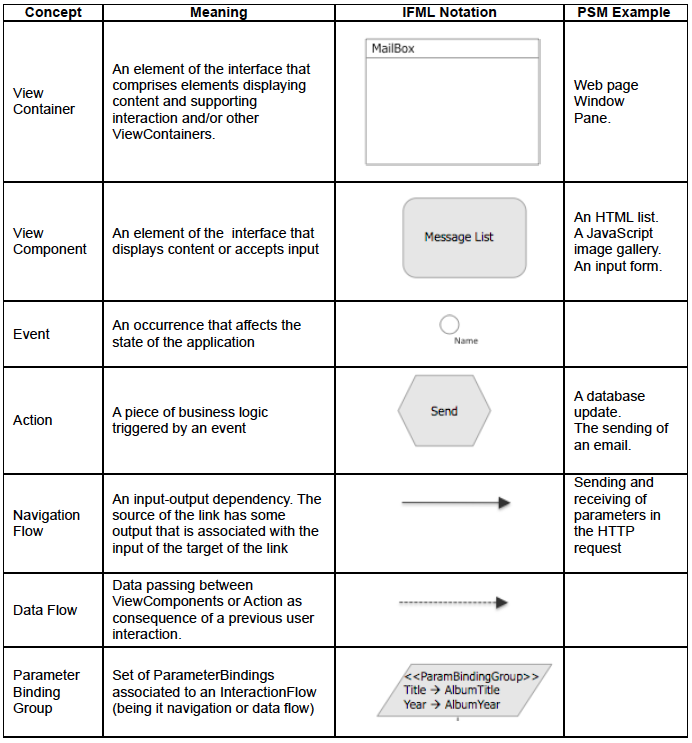
\includegraphics[width=10cm]{images/ifml.jpg}
  \caption{Main IFML concepts and notations.}
  \label{fig:ifml}
\end{figure}
\vspace{0.5cm}

\newpage

\section{Navigational modeling for the Web}

eCommerce website front ends are usually built using shared and reusable components (forms, list views, detail views, etc.) which have a specific and expected behavior.
For example, Product lists and grids show record details for the user to view and interact with an action on these, "Add To Cart" call-to-action buttons are presented within product pages to trigger a different response and so on.
All these interactive operations can be represented using the IFML notation.

To demonstrate the versatility and adaptability of this modeling language we introduce a real-life example which we will use as a reference from this chapter forward: an online boutique website called \textit{"Madison Island"} specialized in fashion items running on an eCommerce platform.

Madison Island presents all the features of a typical eCommerce digital store including navigation and browsing of its catalog, product searching, customer account section, shopping cart and order processing. 


\vspace{0.5cm}
\begin{figure}[htbp]
  \centering
    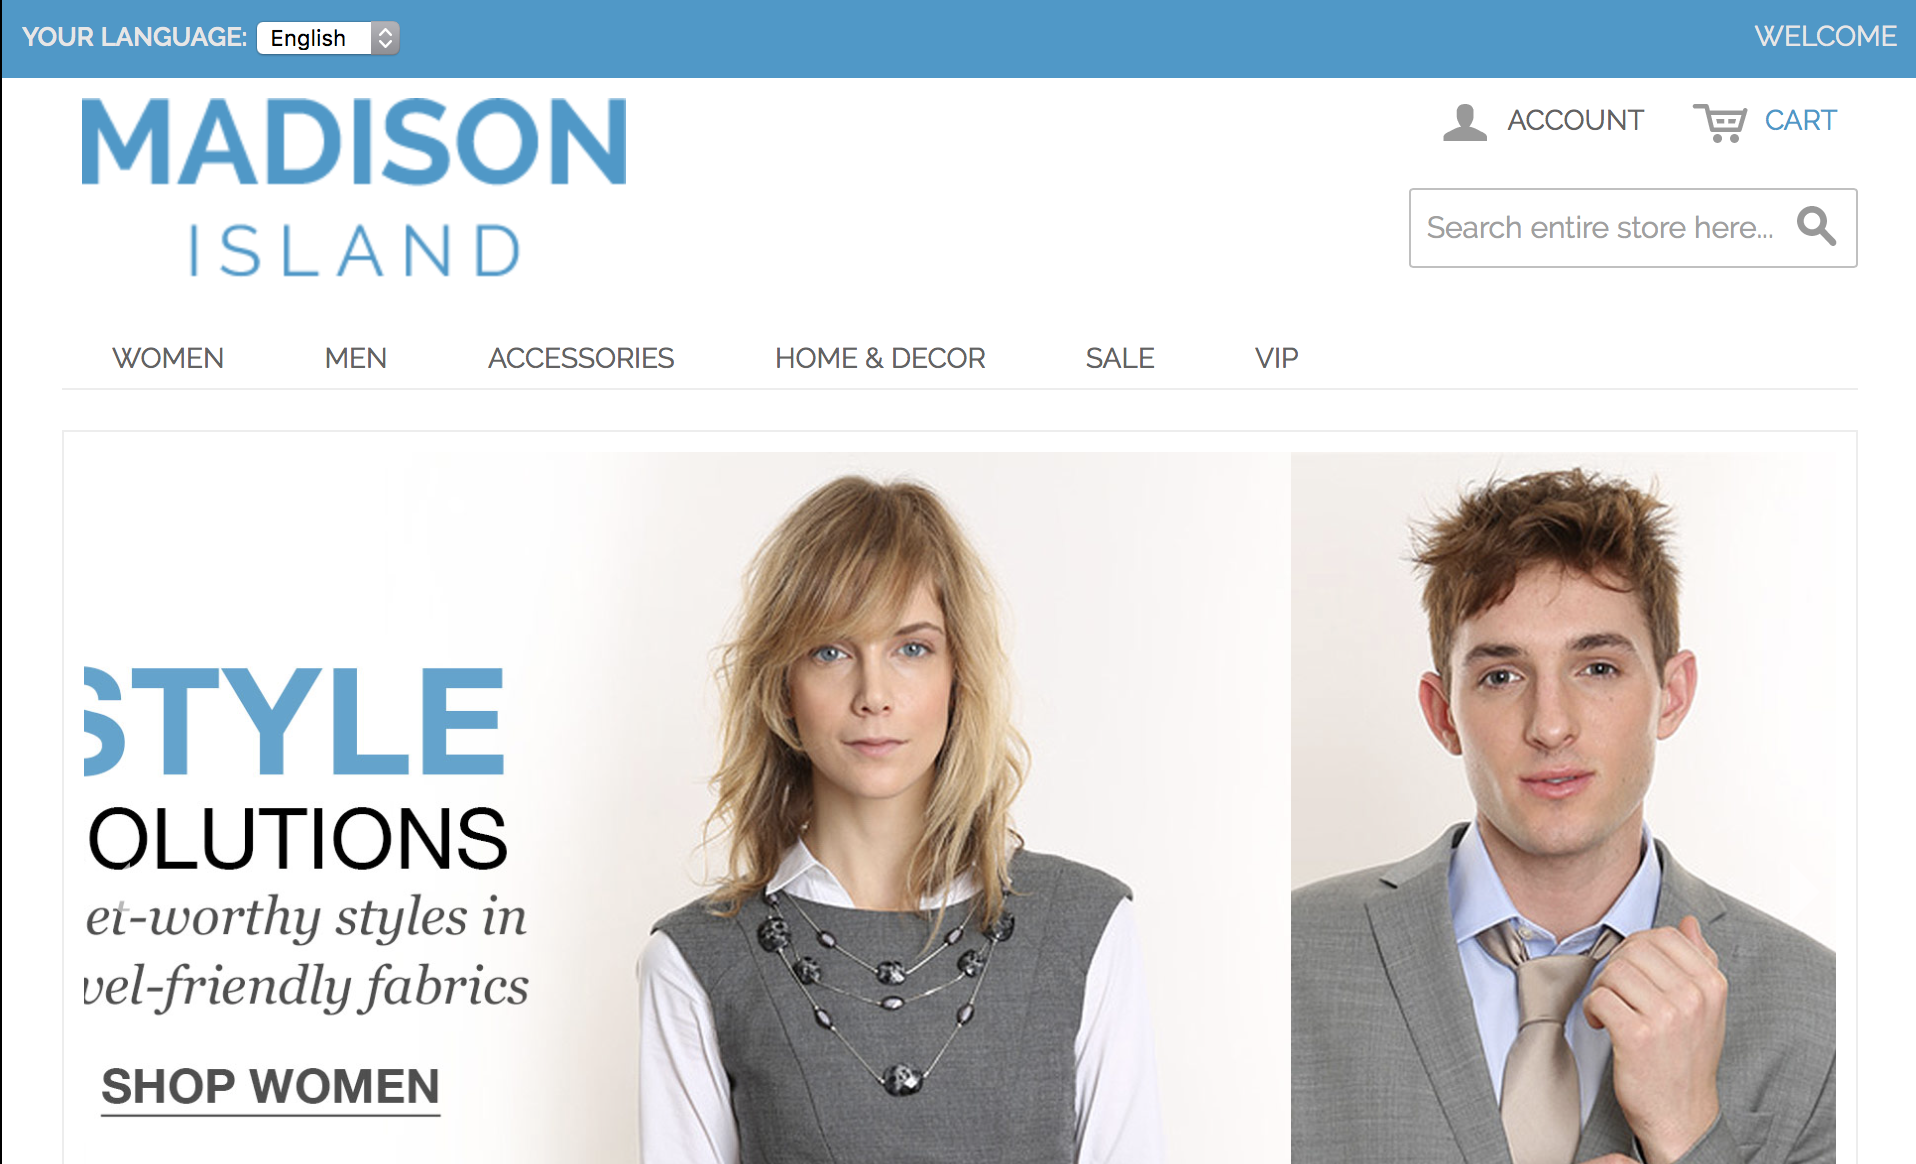
\includegraphics[width=12cm]{images/home.png}
  \caption{Madison Island digital store homepage}
  \label{fig:home}
\end{figure}
\vspace{0.5cm}


Figure \ref{fig:home} shows the home page of the website. In this section, the user can select one of the product categories, access his customer area, switch the language of the website, search for an item or go directly to the shopping cart. 

In the following subsections, we analyze a couple of scenarios related to users navigational behaviors exposing both their representation in IFML notation and the associated server log entries in the application server.

\newpage
\subsection{The product page journey}

Starting from the homepage the user can interact with the navigation menu to select from a set of categories available.  (Figure \ref{fig:navigation})

\vspace{0.5cm}
\begin{figure}[H]
  \centering
    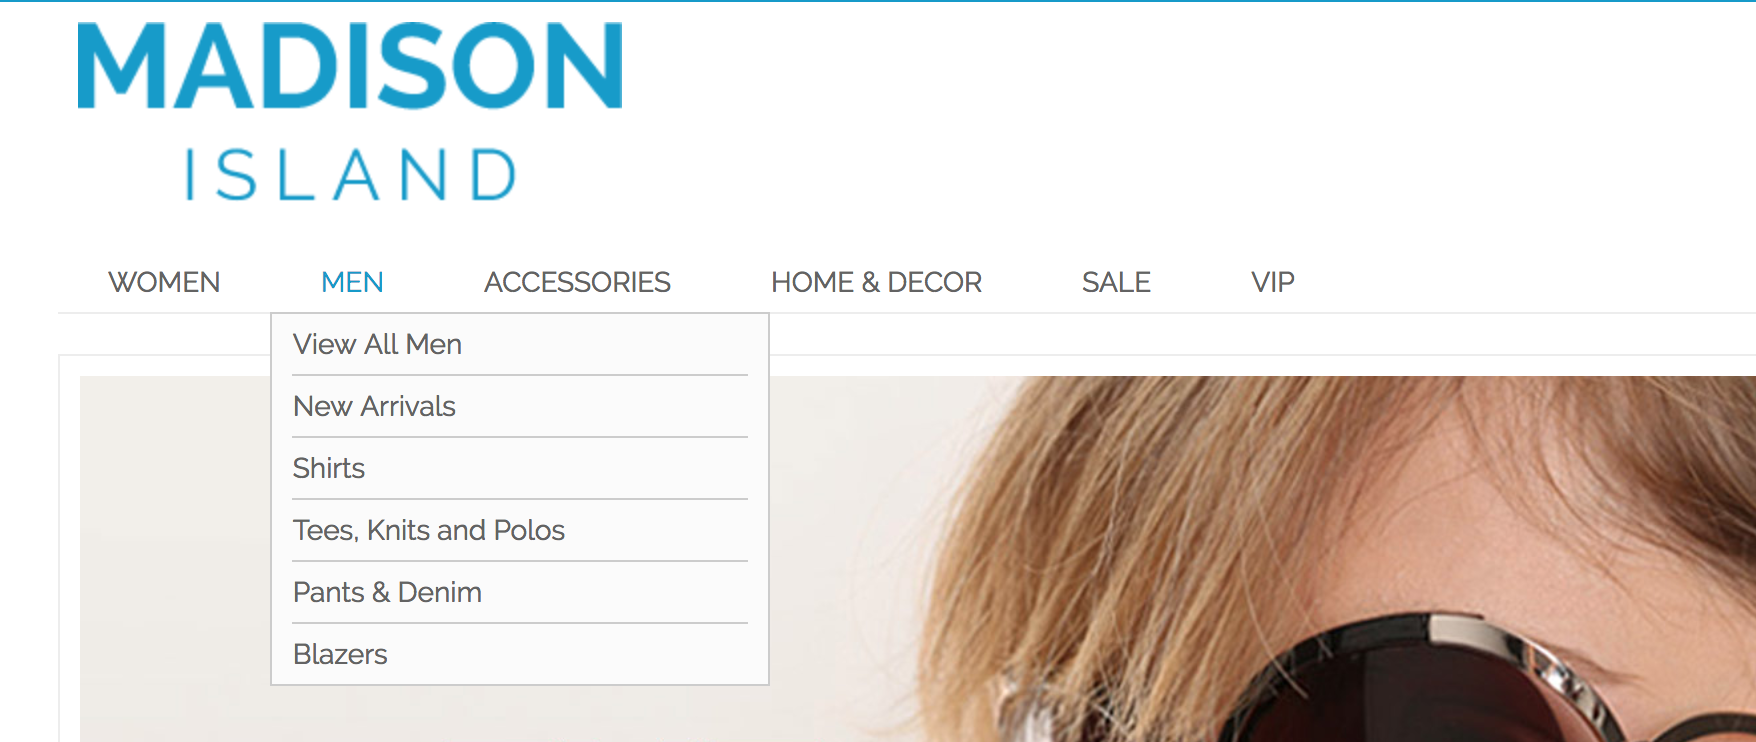
\includegraphics[width=9cm]{images/madison/navigation.png}
  \caption{Navigation menu}
  \label{fig:navigation}
\end{figure}
\vspace{0.5cm}

Depending on the category display mode, a category page can either list CMS content showing a list of links to children categories serving as an intermediary transitional page or directly present its products to the user.
(Figure \ref{fig:category-display-modes})


\vspace{0.5cm}
\begin{figure}[H]
  \centering
  \subfloat[Category listing]{{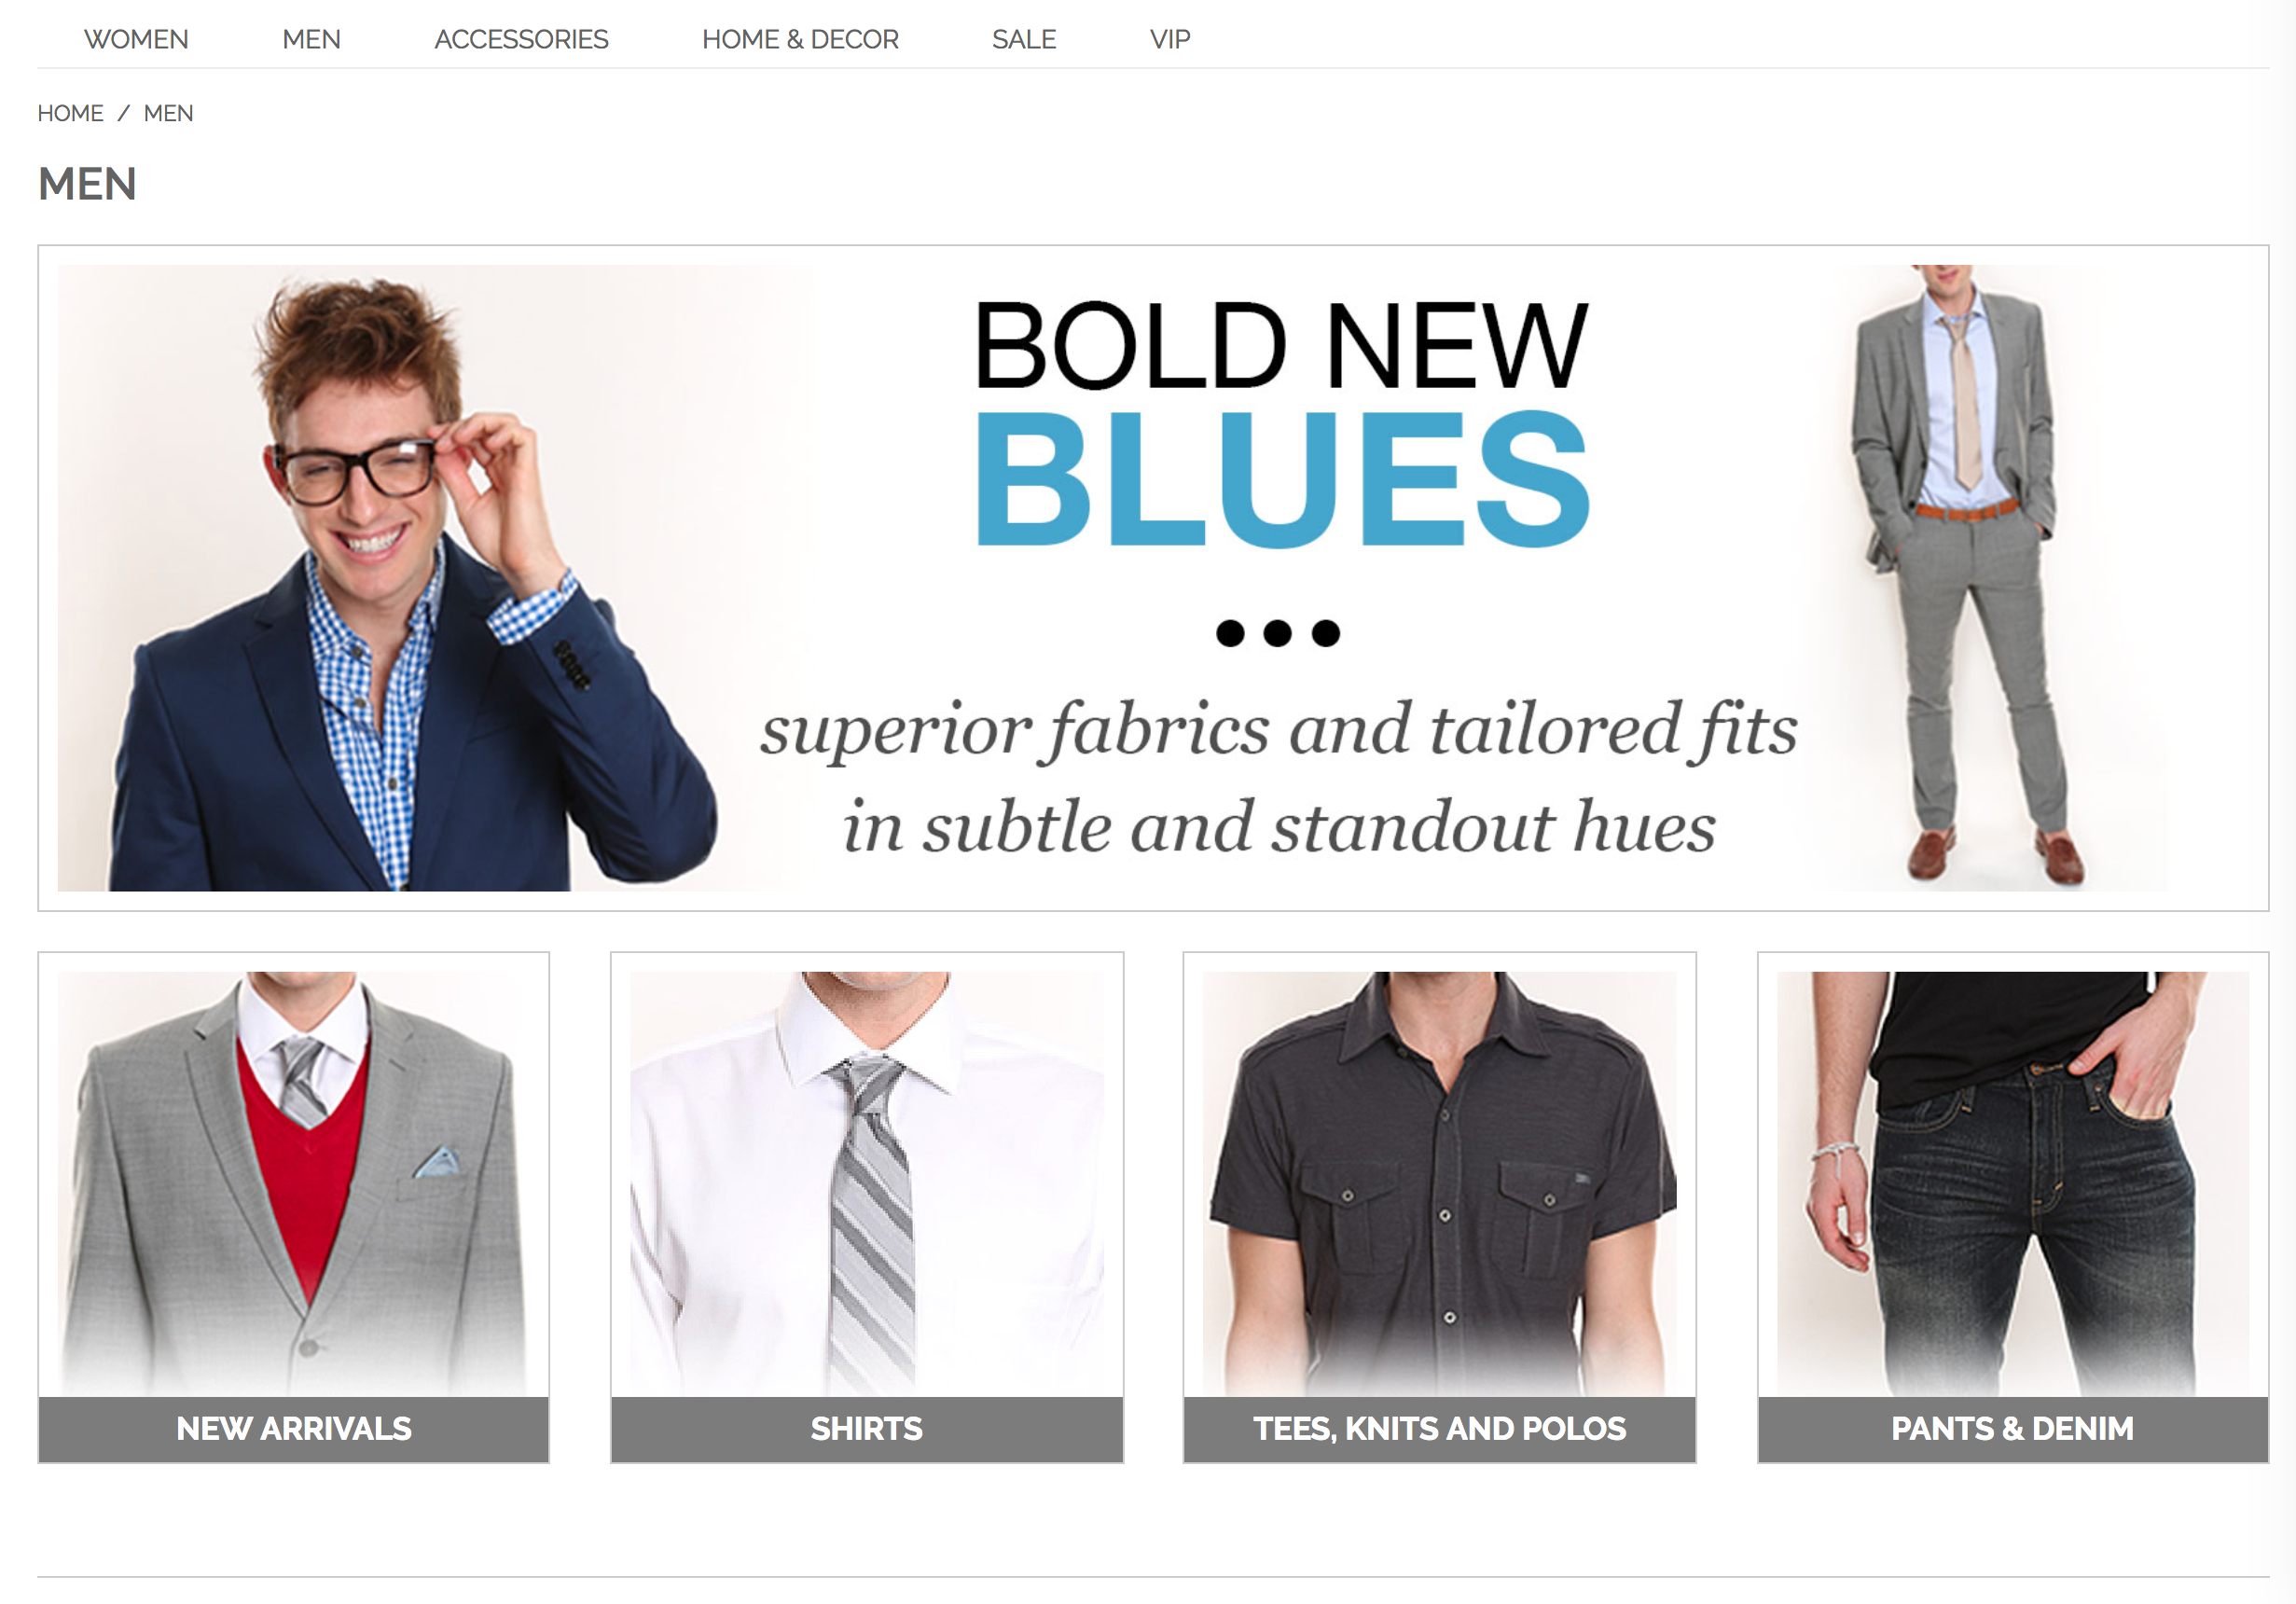
\includegraphics[width=7cm]{images/madison/category-cms.png} }}%
  \qquad
  \subfloat[Product listing]{{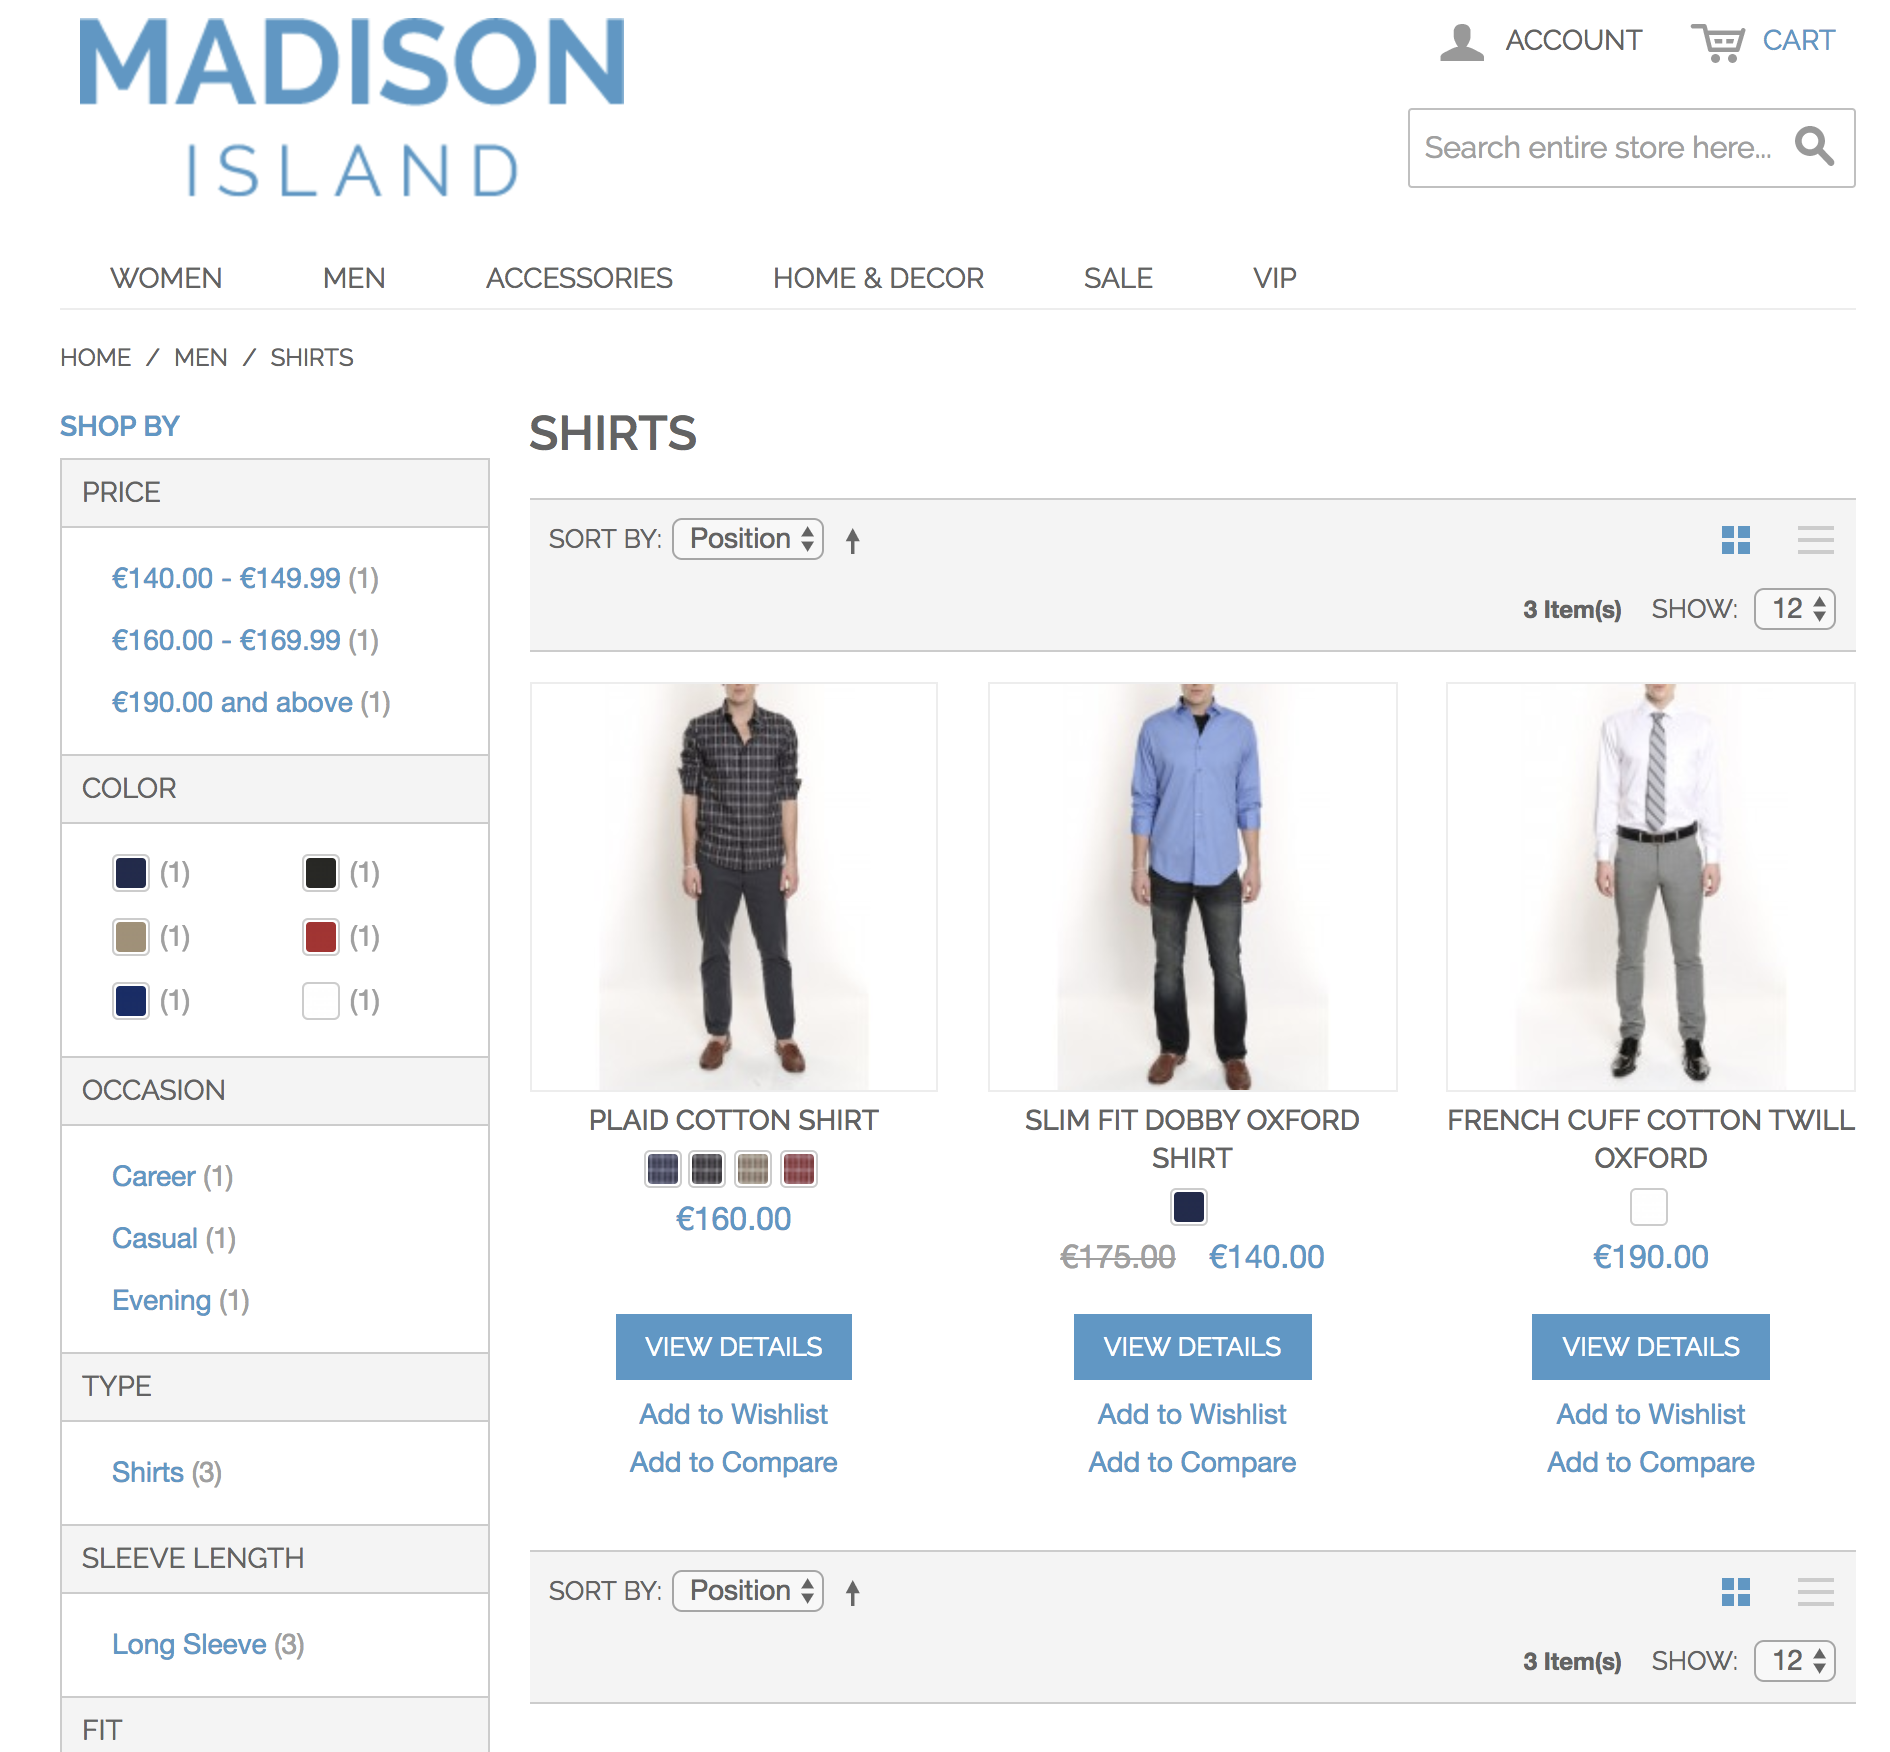
\includegraphics[width=7cm]{images/madison/products-list.png} }}%
  \caption{Different category page view modes}%
  \label{fig:category-display-modes}%
\end{figure}
\vspace{0.5cm}

Finally, from the product listing screen, the user can potentially access any of the product detail pages clicking on the call to action \textit{te"View Details"} below the selected product image thumbnail, let's assume he chooses the \textit{"Plaid Cotton Shirt"} in this case.  
(Figure \ref{fig:product-detail})

\vspace{0.5cm}
\begin{figure}[H]
  \centering
    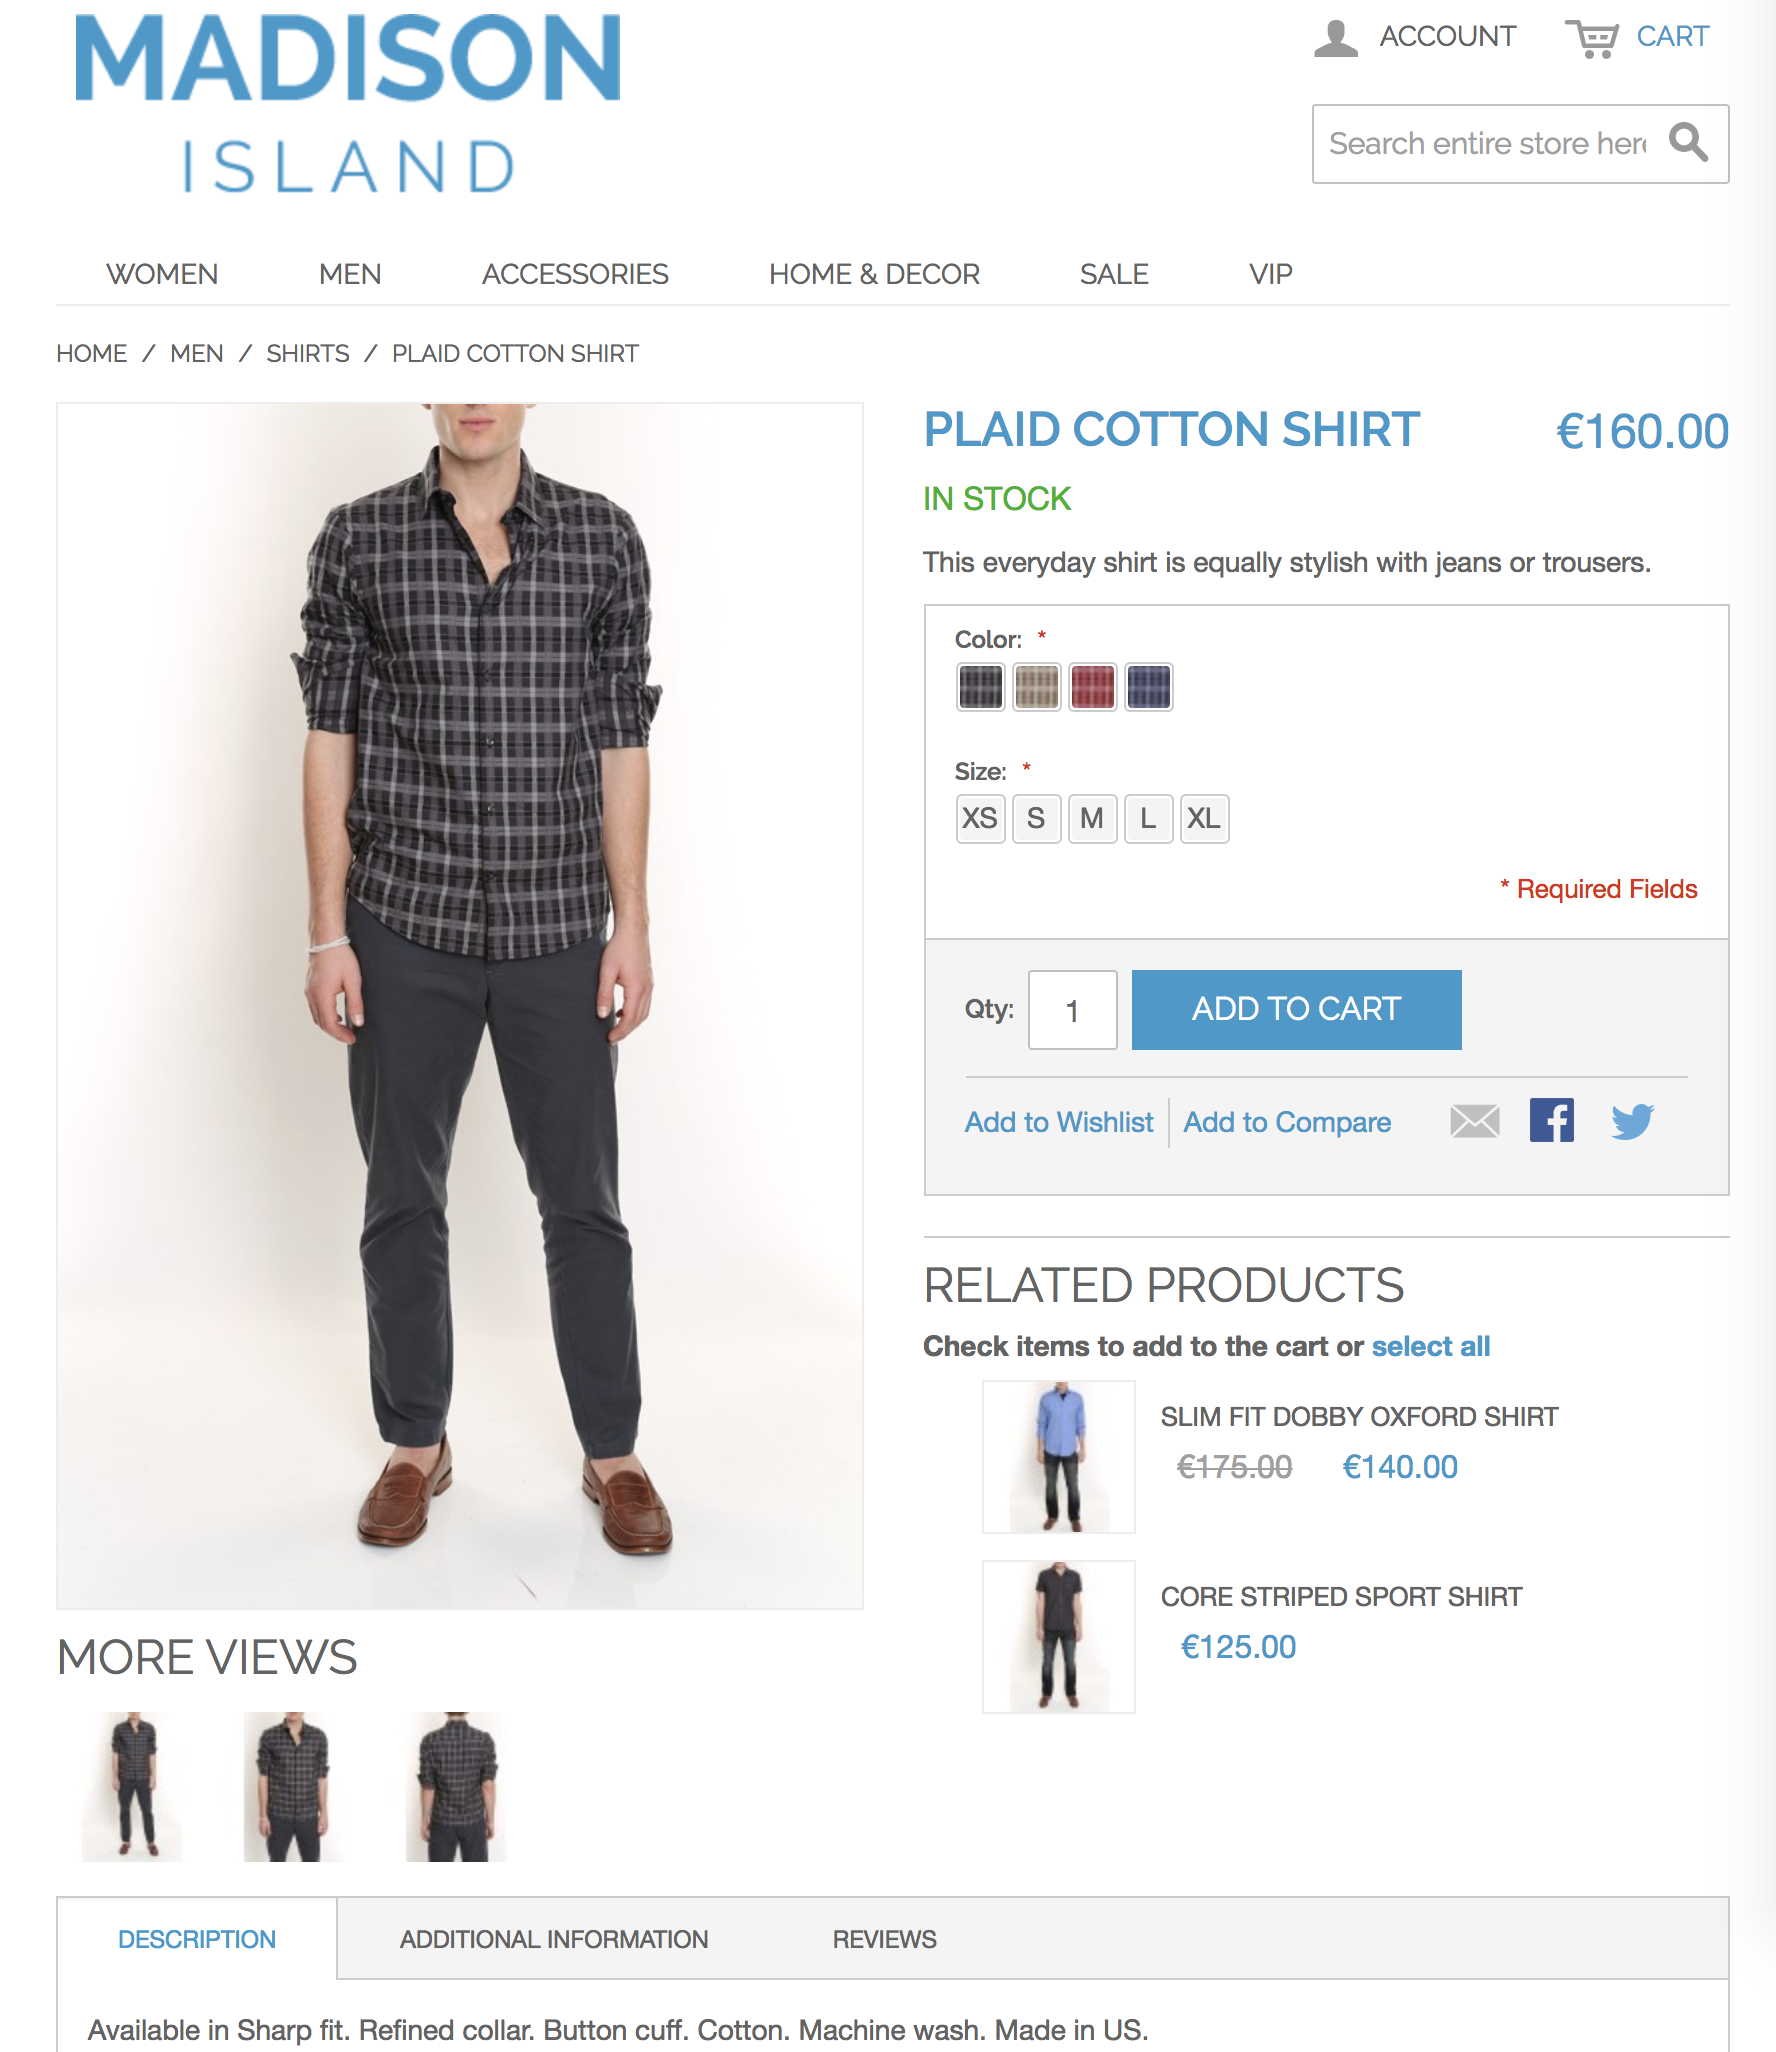
\includegraphics[height=8cm]{images/madison/product-detail.png}
  \caption{Product detail page}
  \label{fig:product-detail}
\end{figure}
\vspace{0.5cm}

The end to end interaction from the homepage to the product detail page can be represented with a model using the following IFML notation:

\vspace{0.5cm}
\begin{figure}[H]
  \centering
    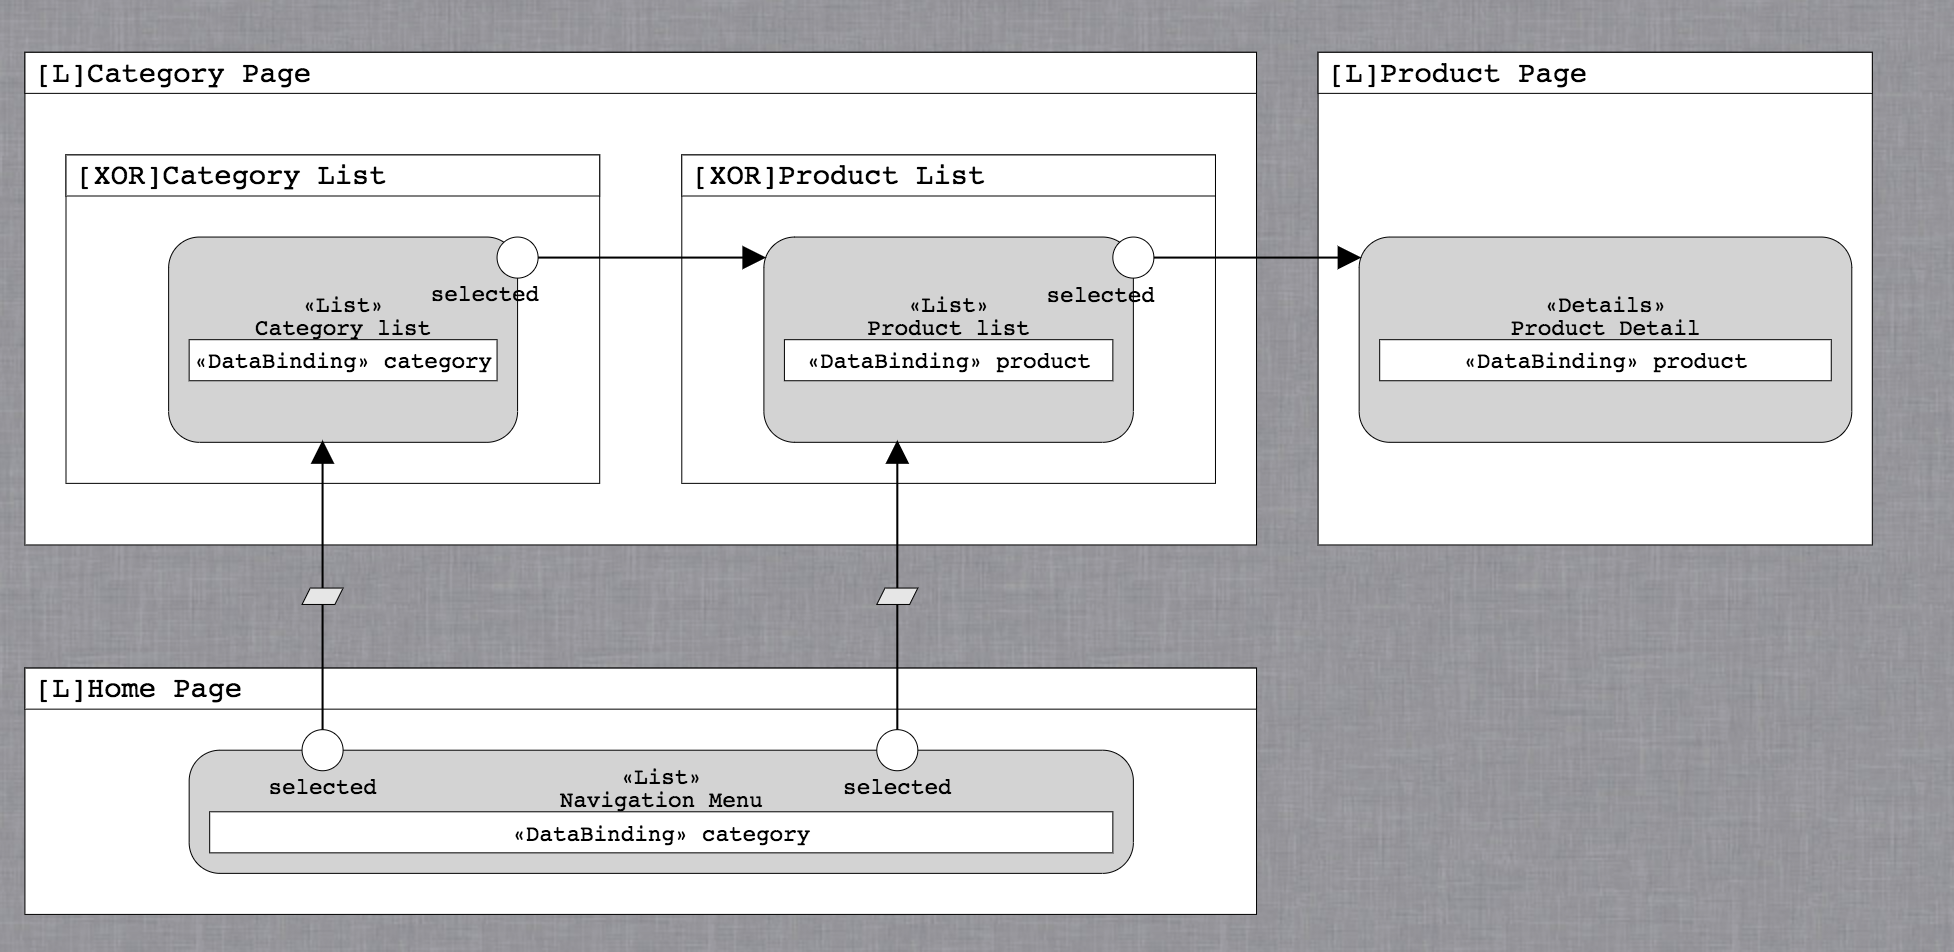
\includegraphics[width=12cm]{images/madison/ifml1.png}
  \caption{IFML representation of the Product Detail interaction}
  \label{fig:ifml1}
\end{figure}
\vspace{0.5cm}

The very same sequence of actions can be expressed as a stream of records in the application server access logs which purpose is to track all the requests processed by the web platform. Here's an example of  the very same user journey we just outlined above :

\vspace{0.5cm}
\begin{center}
  \begin{tabular}{|c|p{3cm}|c|p{6cm}|}
  \hline
  \multicolumn{4}{|c|}{Application Server Access Log}\\ \hline
  \textbf{ID}&\textbf{Page}&\textbf{IFML}&\textbf{Log Entry}   \\ \hline
  1&Home Page&Home&\em[29/Nov/2017:06:30:45 +0000] "GET /" 200 0 - 29505 \\ \hline
  2&\textit{"View All Men"} Category Page &Category&\em[29/Nov/2017:06:49:38 +0000] "GET /men.html /" 200 0 - 29505 
  \\ \hline
  3&\textit{"Shirts"} Category Page &Category&\em[29/Nov/2017:07:04:15 +0000] "GET /men/shirts.html" 200 0 - 29505
  \\ \hline
  4&\textit{"Plaid Cotton Shirt"} Product Page &Product&\em[29/Nov/2017:07:08:40 +0000] "GET /men/shirts/plaid-cotton-shirt-476.html" 200 0 - 29505
  \\ \hline
  \end{tabular}
  \end{center}
  \vspace{0.5cm}

  As noticeable from this table, both entries 2 and 3 record a \textit{"Category Page"} pageview action logging their associated URLs. The entry 4, on the other side, tracks a \textit{"Product Page"} visit by logging a specific URL into the system concatenating the product URL key and the category path for the product itself to flag its direct access from a Category Page.


\subsection{Products association and correlation}

In this scenario, we analyze the set of actions that can possibly generate page views among different product pages on the Madison Island website. 

Using as a starting point the same product page for the \textit{"Plaid Cotton Shirt"} article of the previous navigational behavior analysis,the customer is presented with a \textit{"Related Products"} widget just below the \textit{"Add To Cart"} segment. The principal purpose of this section is to provide the user with some suggestions about products that can be linked in some way to the current one and generate customer's interest.(Figure \ref{fig:related-products})

\vspace{0.5cm}
\begin{figure}[H]
  \centering
    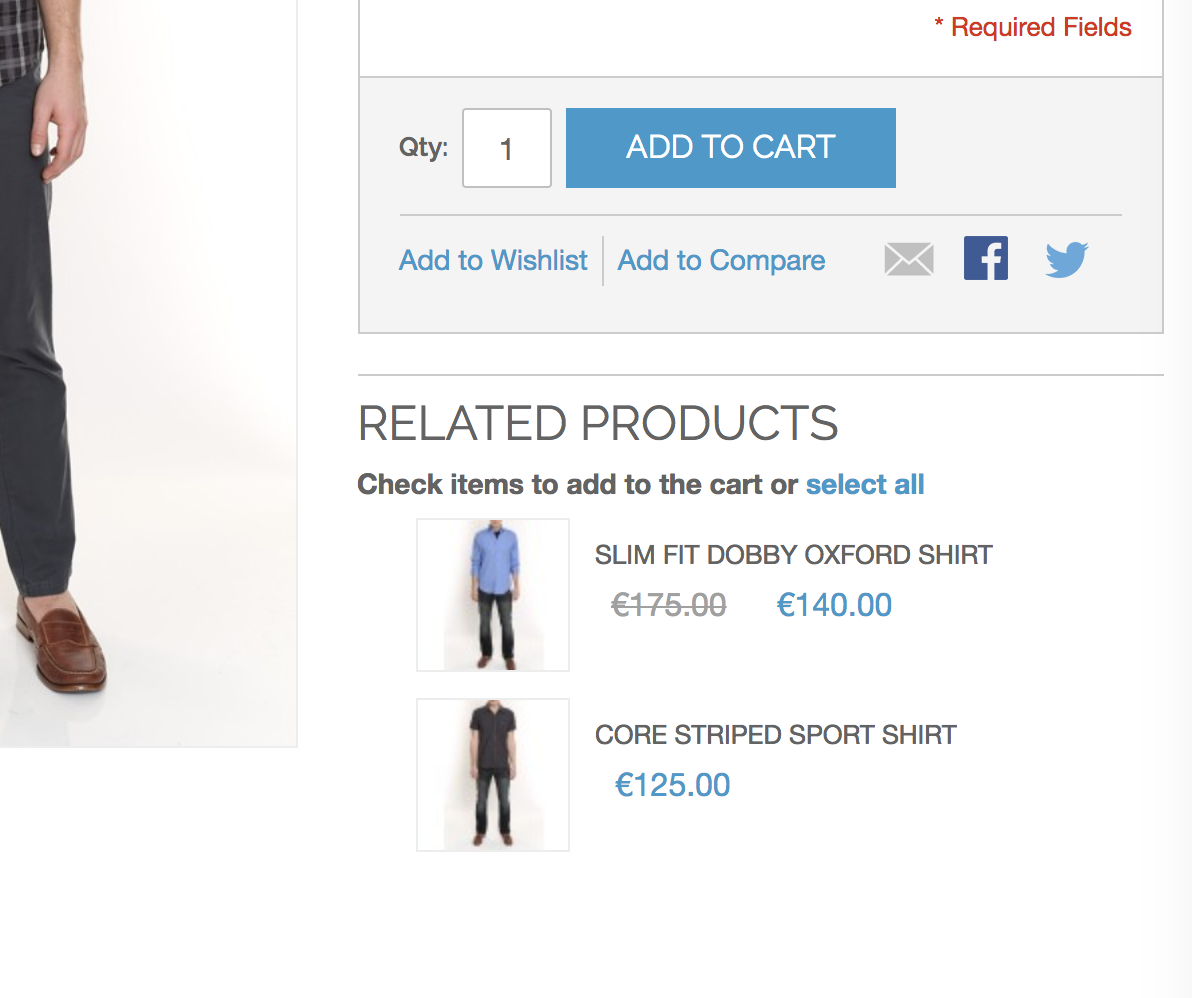
\includegraphics[width=8cm]{images/madison/related-products.png}
  \caption{Related products section}
  \label{fig:related-products}
\end{figure}
\vspace{0.5cm}

Clicking either on the product name or its thumbnail the user is brought to the related product page. In this case, we assume his interest goes for the \textit{"Core Striped Sport Shirt"} item presented in the list. (Figure \ref{fig:product-detail2})

\vspace{0.5cm}
\begin{figure}[H]
  \centering
    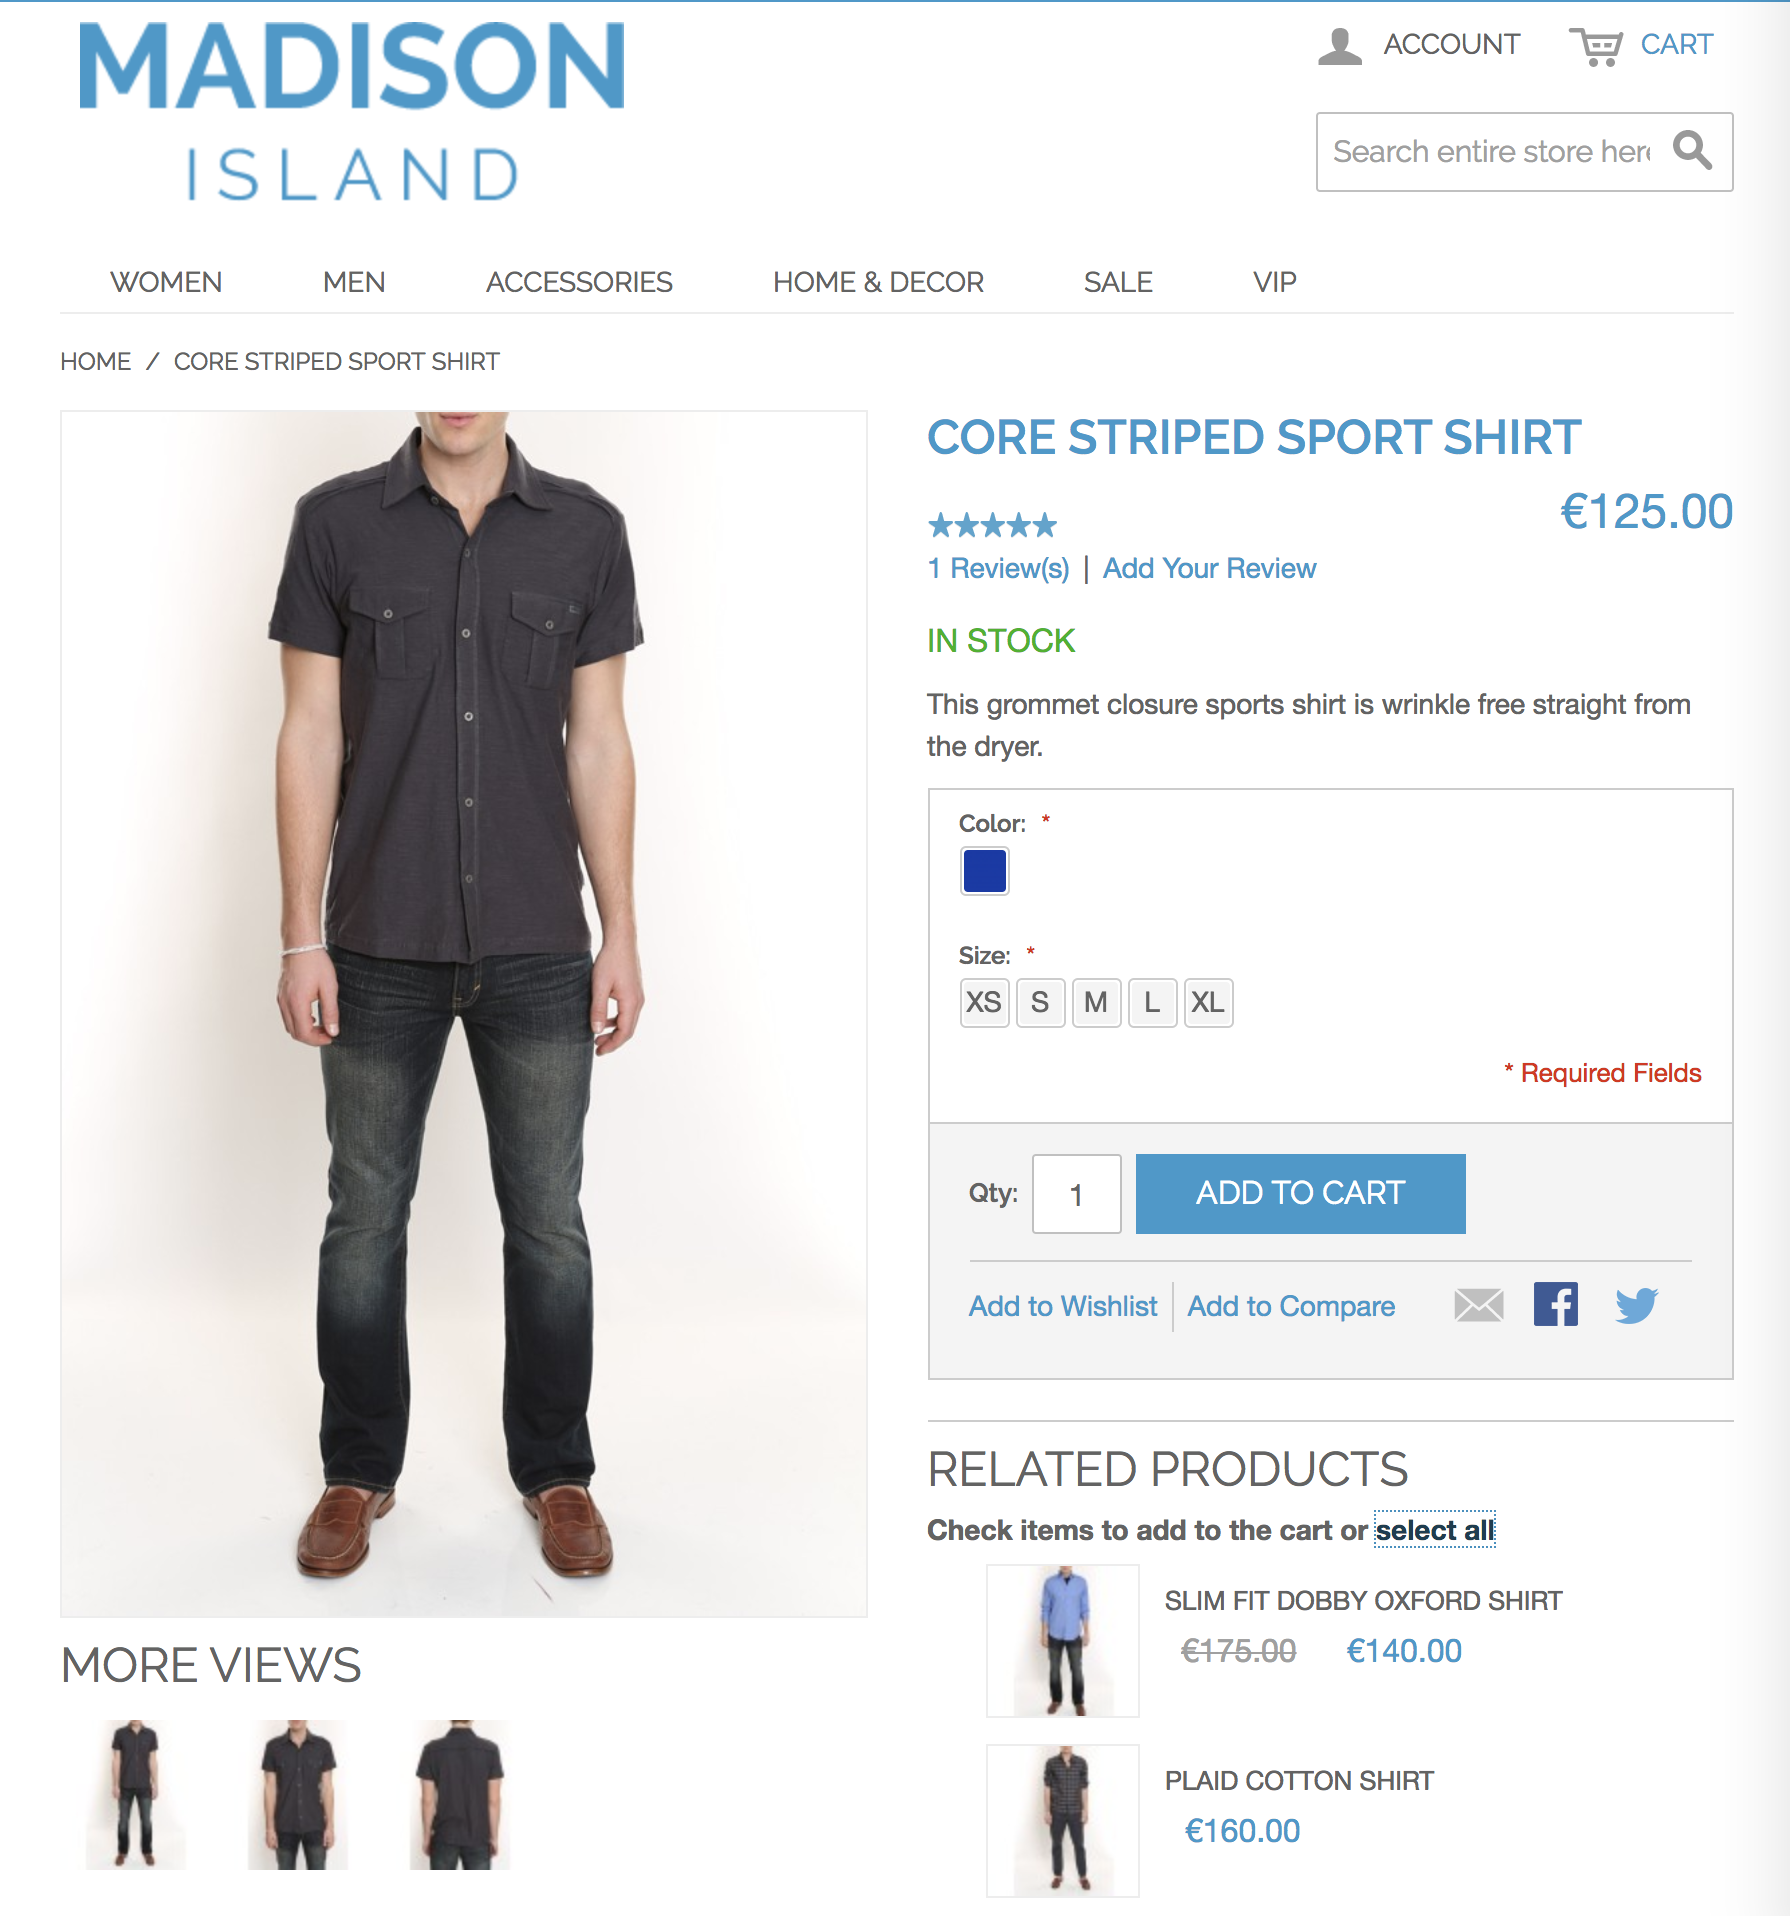
\includegraphics[height=8cm]{images/madison/product-detail2.png}
  \caption{A related product page}
  \label{fig:product-detail2}
\end{figure}
\vspace{0.5cm}

Besides the simple navigational shortcut offered by the related products section, the user can potentially reach a product page in many other alternative ways on the website, the tracking of these interactions could potentially bring benefits for establishing a correlation pattern among the items.  For instance, he can quickly go back with the back button of his browser to the previous category listing page and choose a different item to check, use the navigatoin menu to browse another category or use the search bar on the top bar to perform a global product search. For the sake of this example, we pretend he searches for blazers writing the \textit{"blazer"} word on the previously mentioned search bar from within the current product page. (Figure \ref{fig:product-search})

\vspace{0.5cm}
\begin{figure}[H]
  \centering
    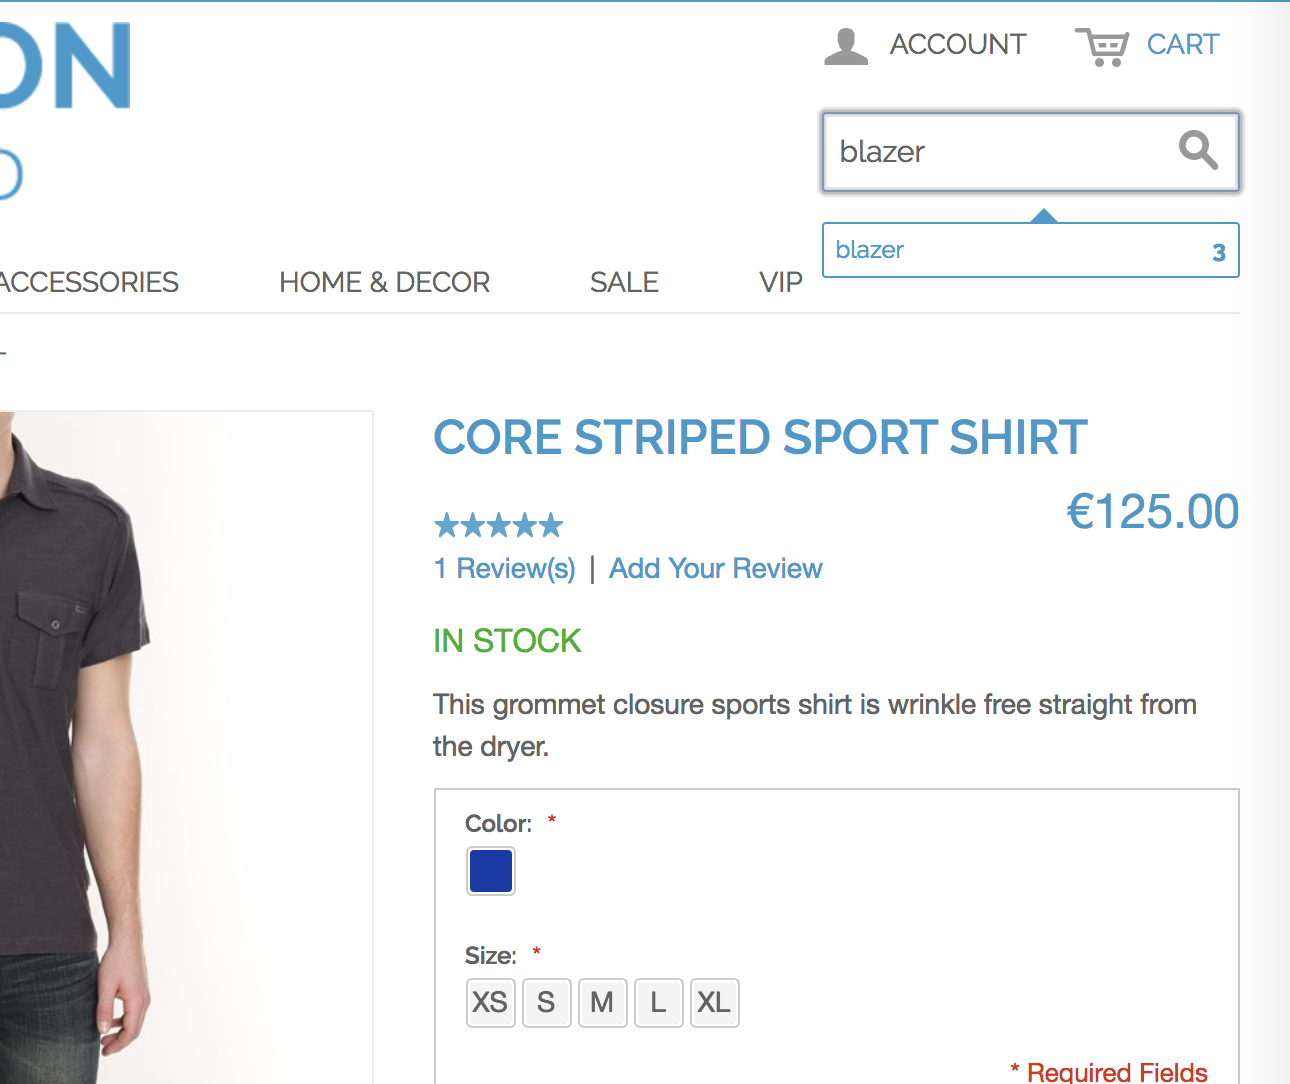
\includegraphics[height=8cm]{images/madison/search.png}
  \caption{Product search bar}
  \label{fig:product-search}
\end{figure}
\vspace{0.5cm}

When the search is performed, the user is taken to the search result page which shows a list of products matching the word he searched for. From within this screen, the user can freely browse to any of the available product pages similarly to what we already described for the category listing page. (Figure \ref{fig:search-results})

\vspace{0.5cm}
\begin{figure}[H]
  \centering
    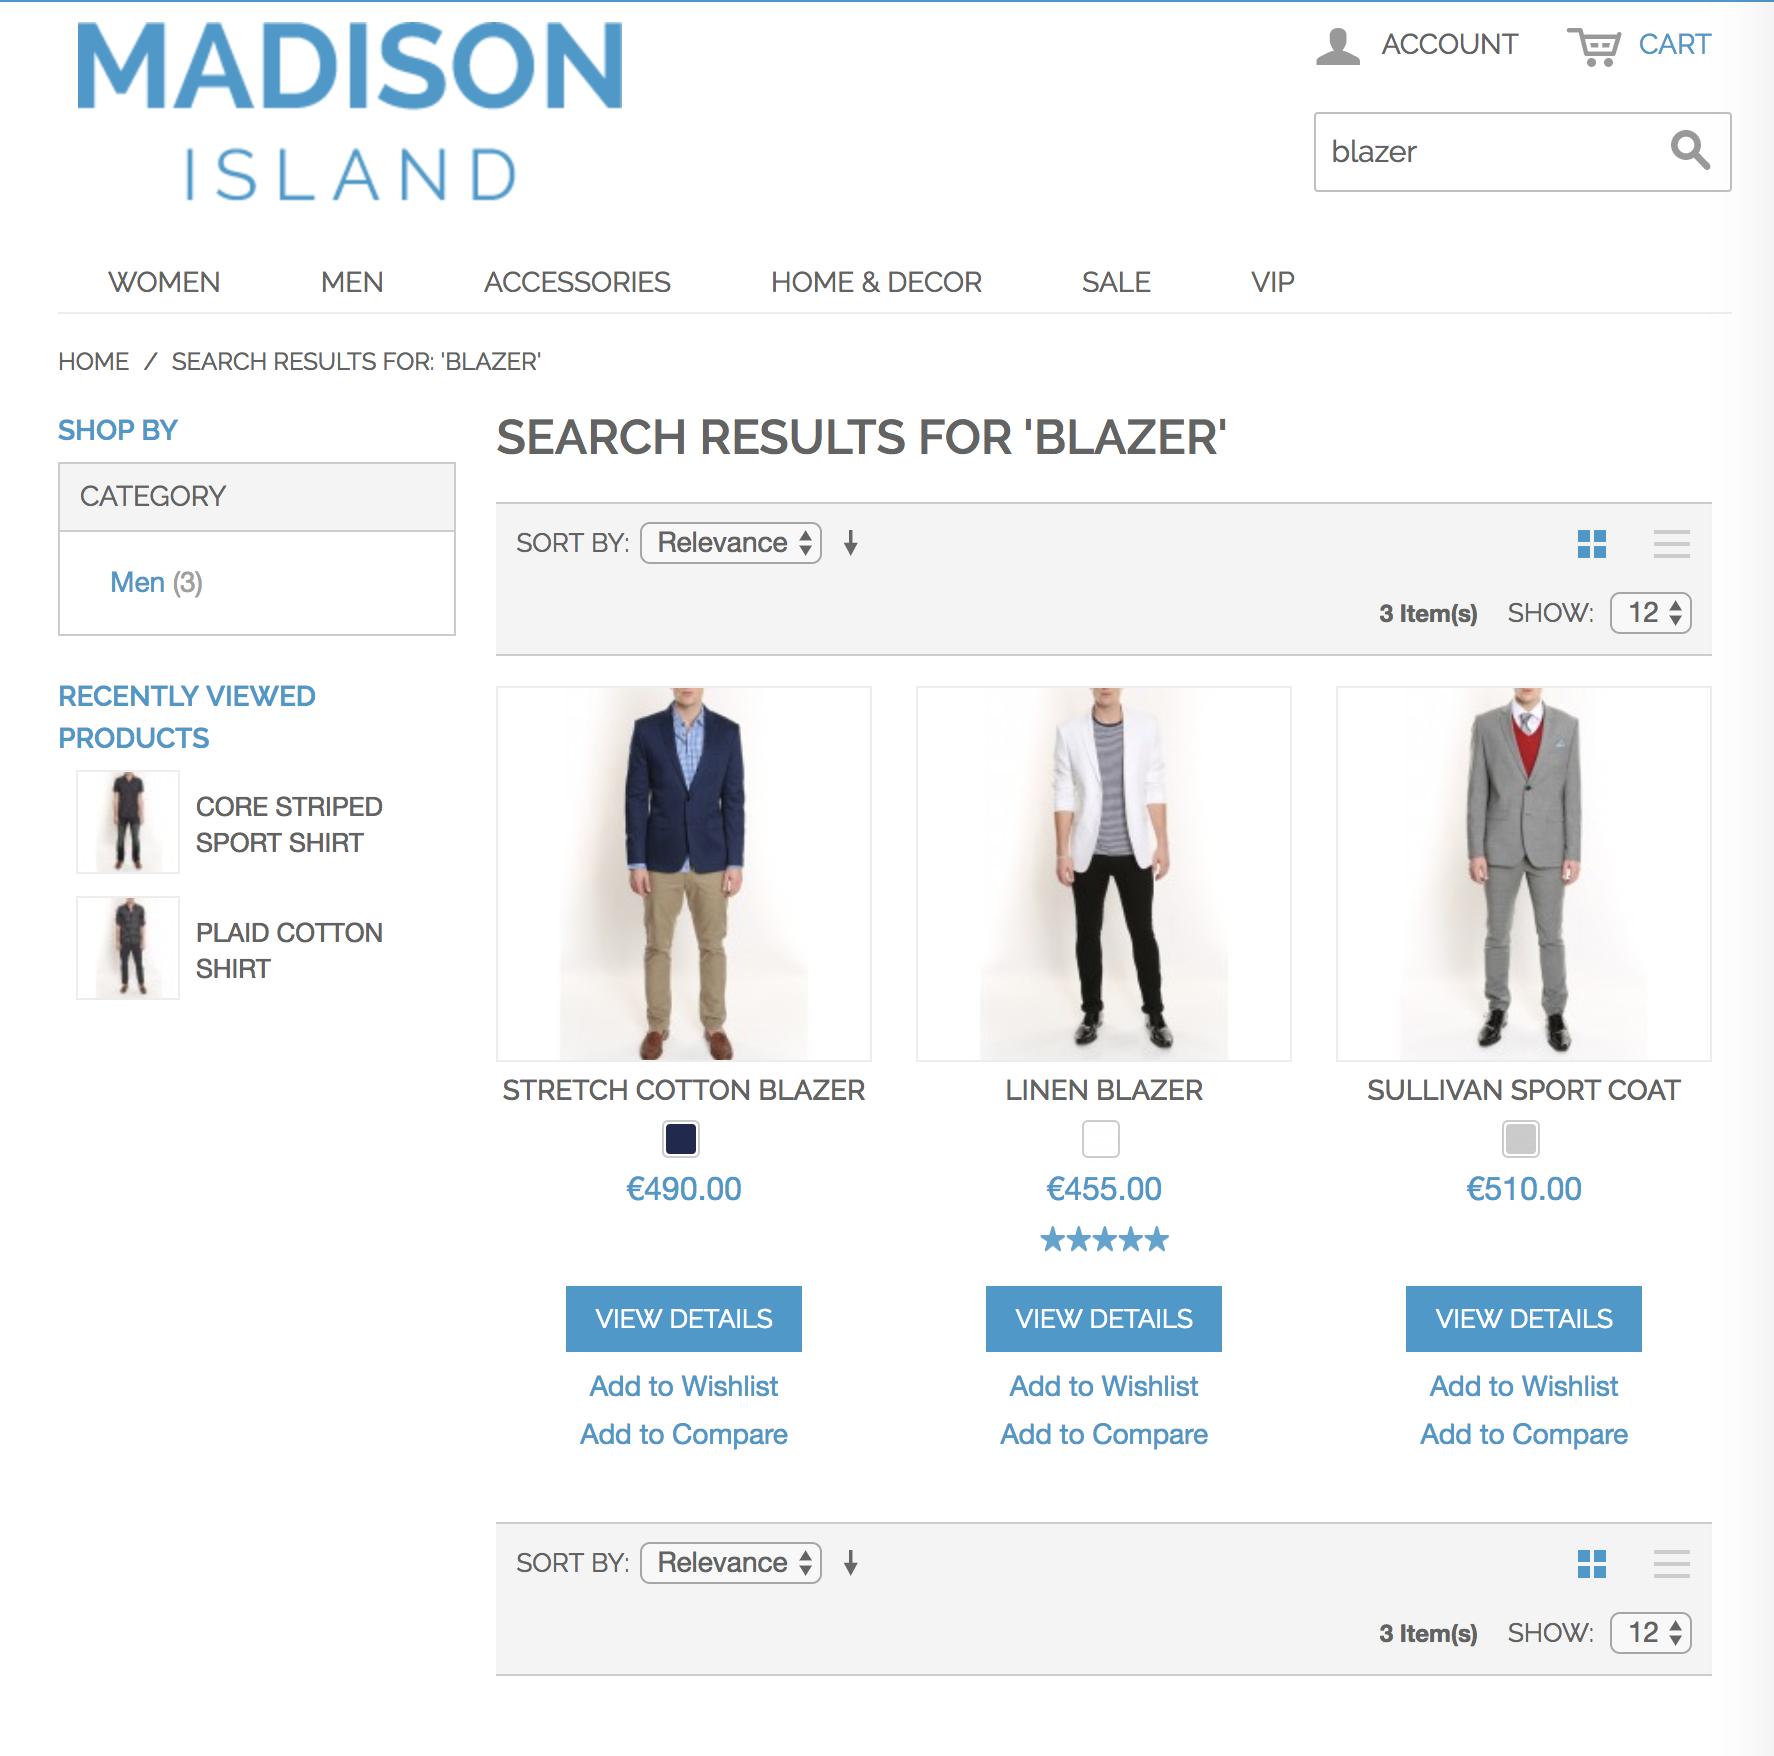
\includegraphics[height=8cm]{images/madison/search-results.png}
  \caption{Search results page}
  \label{fig:search-results}
\end{figure}
\vspace{0.5cm}

At this point, we can update and extend the IFML model shown previously in Figure \ref{fig:ifml1} accordingly to the new notions and interactions that have been described just above.

\vspace{0.5cm}
\begin{figure}[H]
  \centering
    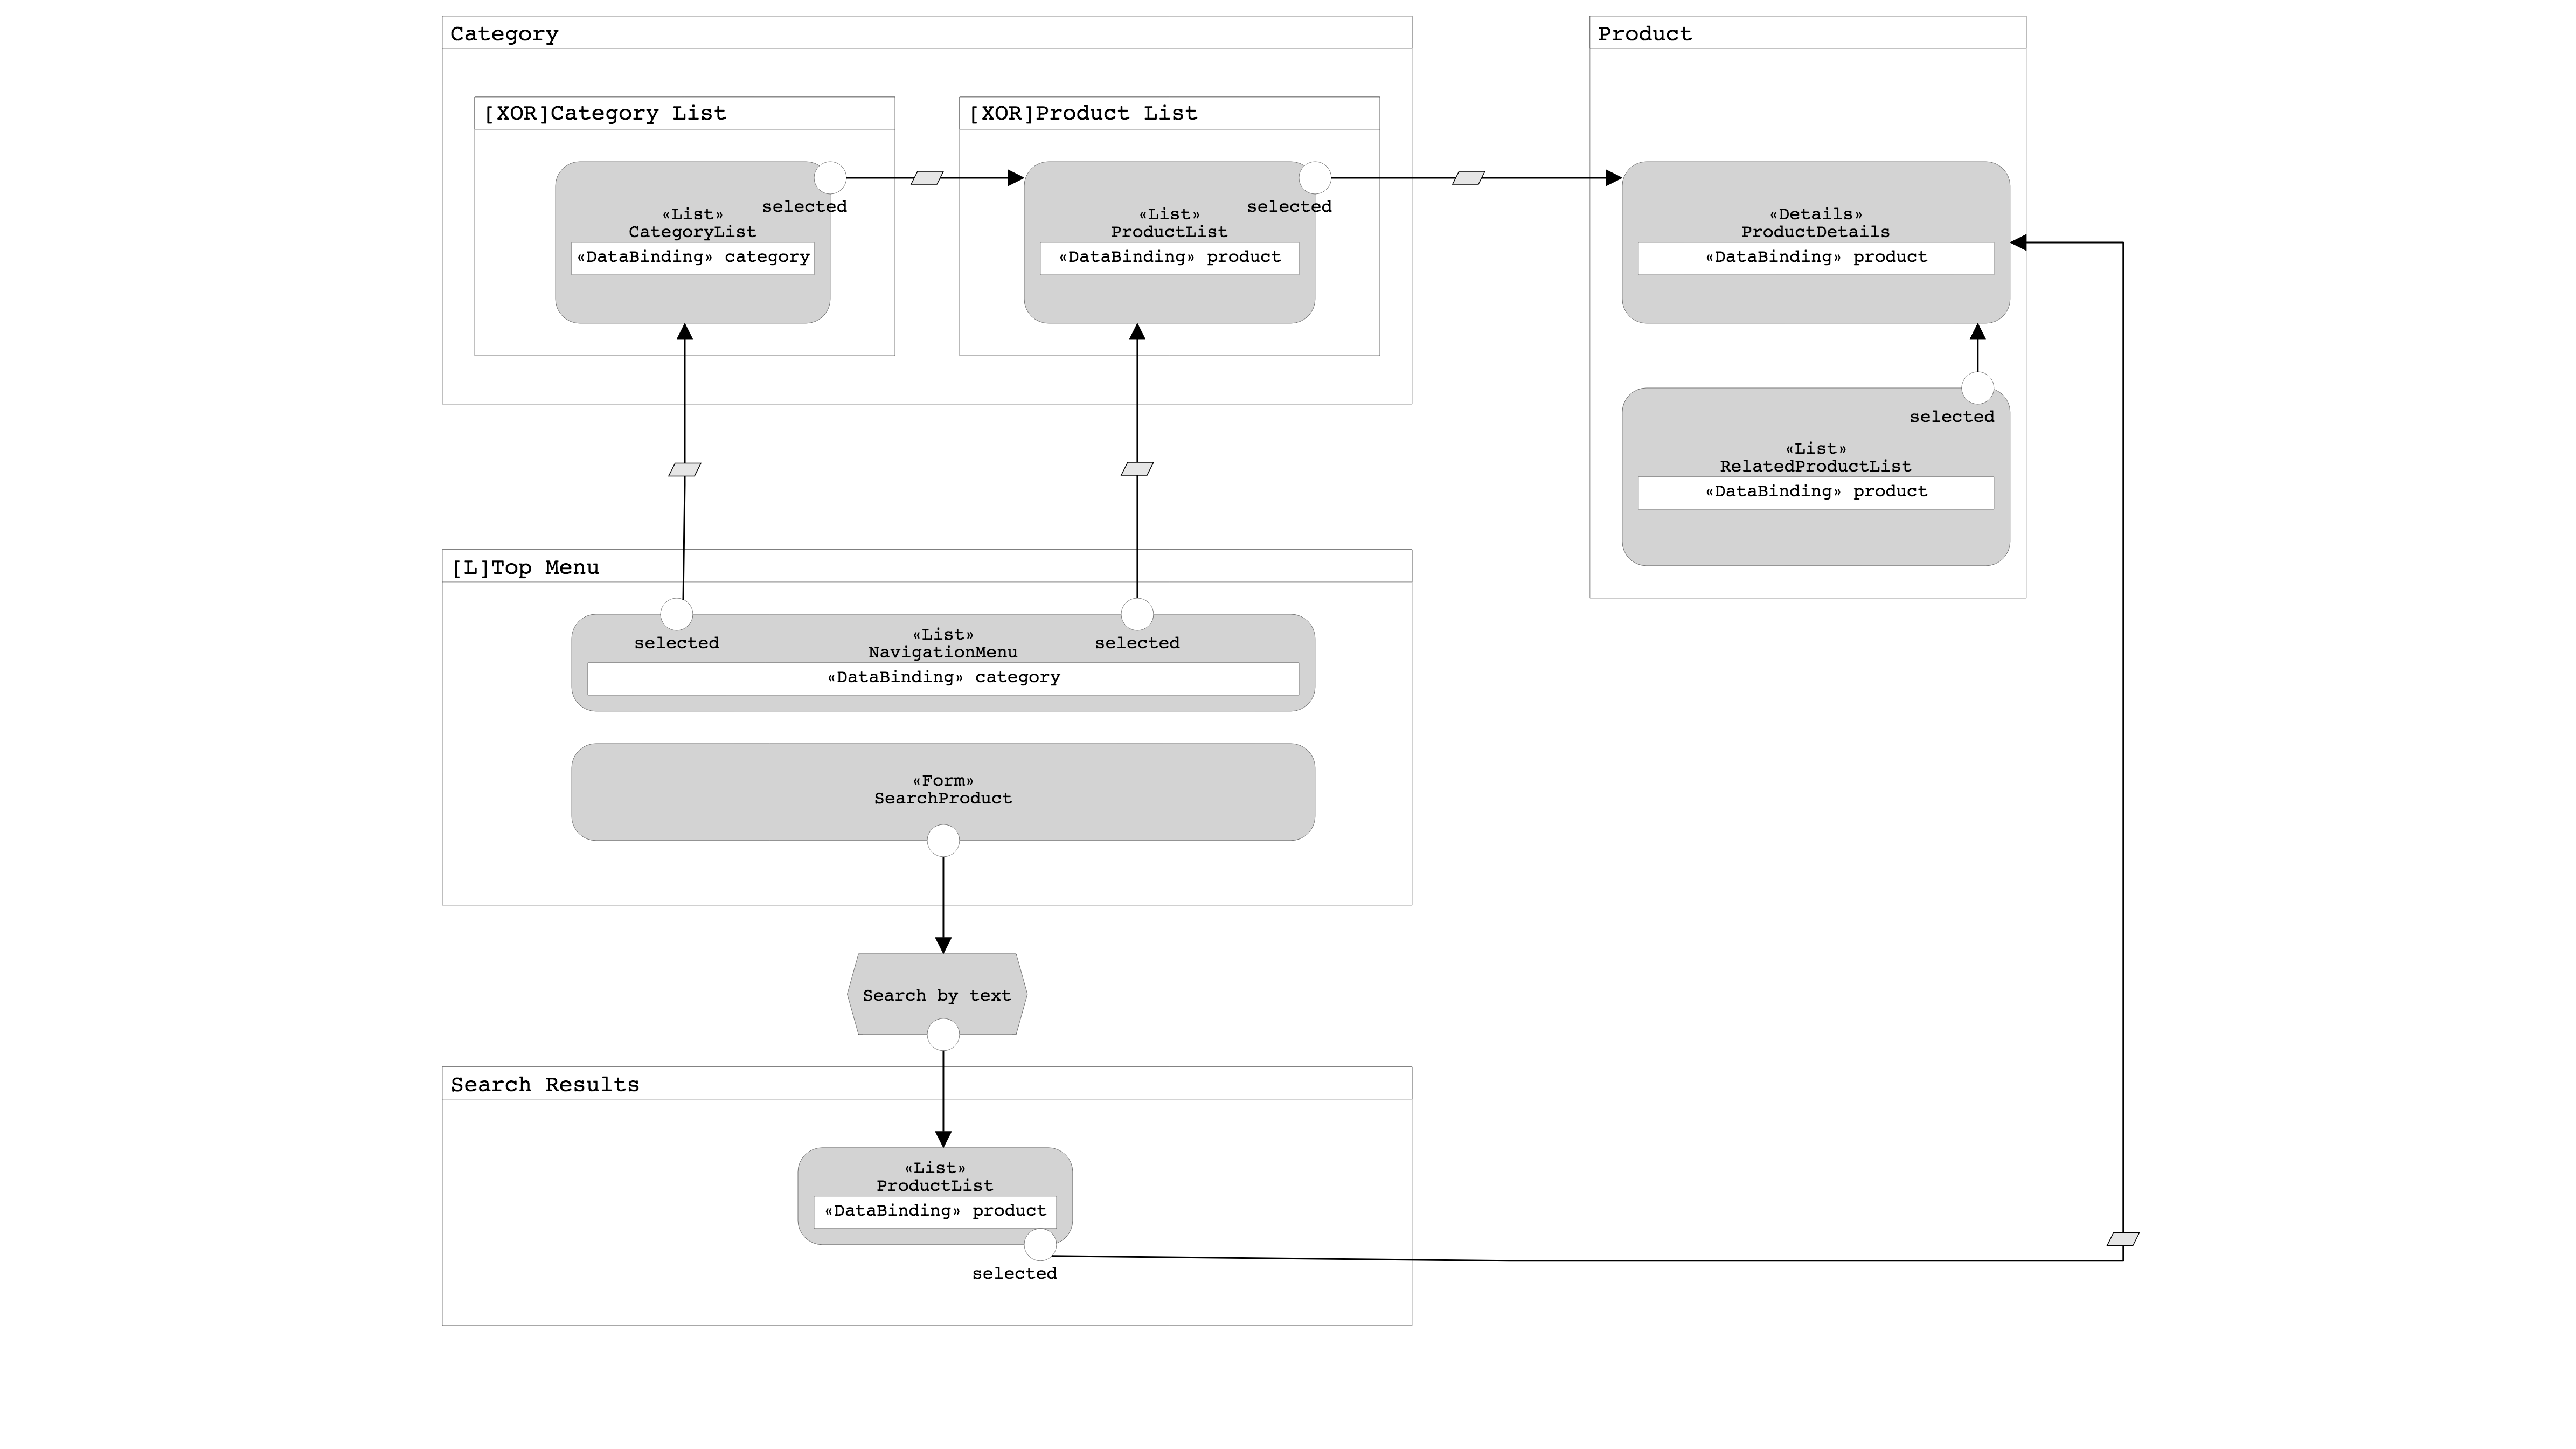
\includegraphics[width=16cm]{images/madison/ifml2.png}
  \caption{Updated IFML representation of the navigational behavious}
  \label{fig:ifml2}
\end{figure}
\vspace{0.5cm}

The same new navigational paths discovered are represented in the application server access log in the following form : 

\vspace{0.5cm}
\begin{center}
  \begin{tabular}{|c|p{3cm}|c|p{6cm}|}
  \hline
  \multicolumn{4}{|c|}{Application Server Access Log}\\ \hline
  \textbf{ID}&\textbf{Page}&\textbf{IFML}&\textbf{Log Entry}   \\ \hline
  1&\textit{"Plaid Cotton Shirt"} Product Page&Product&\em[04/Dec/2017:06:37:06 +0000] 
  "GET /men/shirts/plaid-cotton-shirt-476.html" 200 0 - 29505
  \\ \hline
  2&\textit{"Core Striped Sport Shirt"} Product Page &Product&\em [04/Dec/2017:06:37:15 +0000] "GET /core-striped-sport-shirt-551.html" 200 0 - 29505
  \\ \hline
  3&\textit{"Plaid Cotton Shirt"} Product Page &Product&\em[04/Dec/2017:06:37:21 +0000] "GET /men/shirts/plaid-cotton-shirt-476.html" 200 0 - 29505
  \\ \hline
  5&\textit{"Tees Knits And Polos"} Category Page &Category&\em[04/Dec/2017:06:38:06 +0000] "GET /men/tees-knits-and-polos.html" 200 0 - 29505
  \\ \hline
  6&\textit{"Blazer"} Search By Term&Search Results&\em[04/Dec/2017:06:38:20 +0000] "GET /catalogsearch/result/?q=blazer" 200 0 - 29505
  \\ \hline
  7&\textit{"Stretch Cotton Blazer"} Product Page &Product&\em[04/Dec/2017:06:38:43 +0000] "GET /stretch-cotton-blazer-587.html" 200 0 - 29505
  \\ \hline
  \end{tabular}
  \end{center}
\vspace{0.5cm}

The sequence of actions recorded from the access logs reveal the user browsed from one product to another taking advantage of the related product links available (ID 2); in fact, the target URL does not include any category path beside the URL key associated with the product indicating a direct access. The entries 3 and 4 illustrate the journey of the user clicking on its back button on the browser and performing the very same actions again. The last three actions recorded show a direct access to a category page through the usage of the navigational menu, a search by the \textit{"blazer"} term as per the previous example and the related redirection to the product page respectively.

\newpage
\section{IoT behavioral modeling}

With mobile surpassing desktop as the most critical influencer for customers to make purchase decisions and track behaviors, location and proximity tracking is proving to be a valuable tool for brands and stores.  In these two next subsections, we analyze two possible scenarios of customer interaction in the real world based on IoT devices recording and reporting capabilities. The data coming from IoT devices would then be collected in conjunction with the web-based one described previously to form a combined behavioral data stream to leverage for generating tailored customizations of the Madison eCommerce webportal.

\subsection{Apple iBeacon technology and Estimote Beacons overview}

The IoT device of choice to illustrate the scenarios related to the behavioral modeling would be the Estimote Beacons which are using Apple iBeacon technology and are compatible with iBeacon-enabled Apple products and applications.

The company from Cupertino jumped first on the beacon bandwagon publishing a detailed specification (IDs, transmission intervals, etc.) in 2013 developing the iBeacon protocol and unlocking vendors, such as Estimote, to ship iBeacon-compatible hardware transmitters.

\vspace{0.5cm}
\begin{figure}[H]
  \centering
    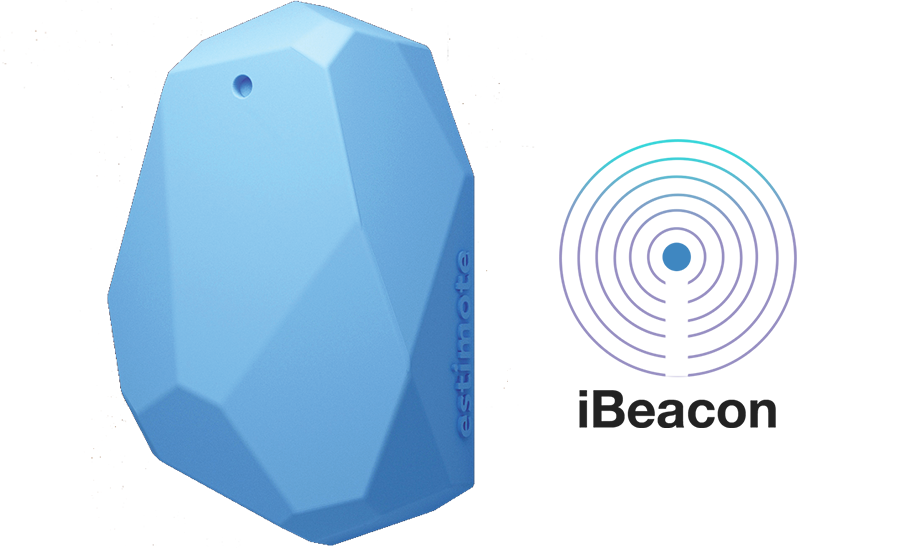
\includegraphics[width=16cm]{images/ibeacon.png}
  \caption{An Estimote iBeacon compatible device}
  \label{fig:estimote-beacon}
\end{figure}
\vspace{0.5cm}

As per previously described in \ref{beacons} a beacon can simply be seen as a lighthouse broadcasting information in certain intervals and at a defined power leveraging Low Energy Bluetooth connection. In the case of iBeacons the information sent to listening mobile devices would contain:


\begin{itemize}
  \item The Universal Unique ID (UUID) is globally unique. Example: de2b45ae-ed98-11e4-3432-78616d6f6f6d
  \item The Major ID uniquely identifies our customer’s system: e.g. 51314
  \item The Minor ID reports the exact location or object (in our case, the spot): e.g. 23369
\end{itemize}

To receive this 1-way data stream the customer needs to have an app installed on his phone unlike QR and NFC communication. Technically, the app obeys only to "its" iBeacons, those with fitting UUID, Major and Minor IDs looking for a match, when this happens the app can react accordingly. This mechanism ensures that only the installed app can track users as they passively walk around the transmitters. 

In detail, the phone OS will keep listening for beacons at all times—even if the app is not running or it was closed, and even if the phone is locked or rebooted. Once an “enter” or “exit” happens, the OS will launch the app into the background (if needed) and let it execute some code for a few seconds to handle the event.

\subsection{Proximity Marketing}
\label{ssection:proximity-marketing}

Proximity Marketing is an efficient tool to involve and discover new potential customers or target better the already existing ones. This marketing technique operates in a given physical location leveraging technologies offered by the IoT ecosystem to promote the sale of products and services.  This communication channel acts on a clear consumer target: all the customers who are in the vicinity or within a given area, covered by the diffusion devices.

This innovative form of relationship marketing aims to activate and involve users by capturing attention at the right time and in the right place, making it experience a more intense and stimulating shopping experience.

In the context of this thesis work, we will focus on a basic scenario where the customer proximity recognition happening in the real world does not directly trigger any immediate action to grab customer attention but it limits itself to silently track the event collecting and sending a communication to a listening web server.

We start defining a possible allocation of items for a "Madison Island" retail store which resembles the catalog presented on its website.

\vspace{0.5cm}
\begin{figure}[H]
  \centering
    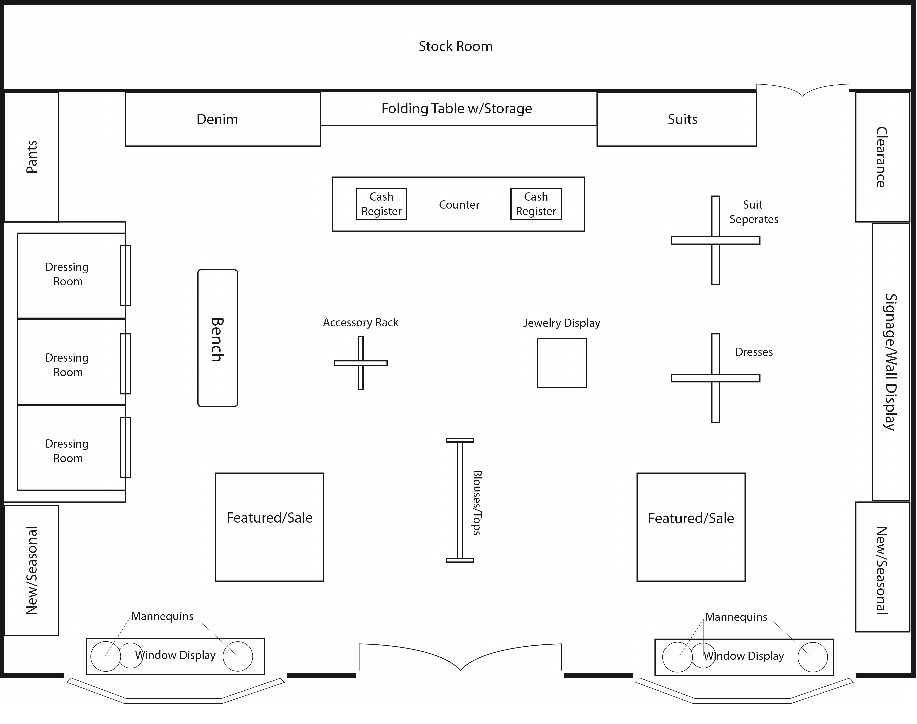
\includegraphics[width=16cm]{images/madison/retail-map.jpg}
  \caption{Madison Island retail store map}
  \label{fig:retail-map}
\end{figure}
\vspace{0.5cm}

Each label described in \ref{fig:retail-map} represents a specific category of the website whereas the color of the label itself indicates the parent category the items belong to. In more detail :

\begin{itemize}
  \item Red categories belong to the \textbf{Women} category mapping the content available at \textbf{/women.html}. 
  \item Blue categories belong to the \textbf{Men} category mapping the content available at \textbf{/men.html}.
  \item Purple categories belong to the \textbf{Home \& Decor} category mapping the content available at \textbf{/home-decor.html}. 
  \item Orange categories belong to the \textbf{Accessories} category mapping the content available at \textbf{/accessories.html}. 
\end{itemize}

As the customer walks around the shop, the Madison Island mobile app will scan for a predefined set of beacon regions and register proximity data whenever the device enters and exits from each one of them efficiently tracking which aisles (regions) customers visited and which not. 

Considering the above, the following would be a suitable Estimote beacon allocation for the store :

\vspace{0.5cm}
\begin{figure}[H]
  \centering
    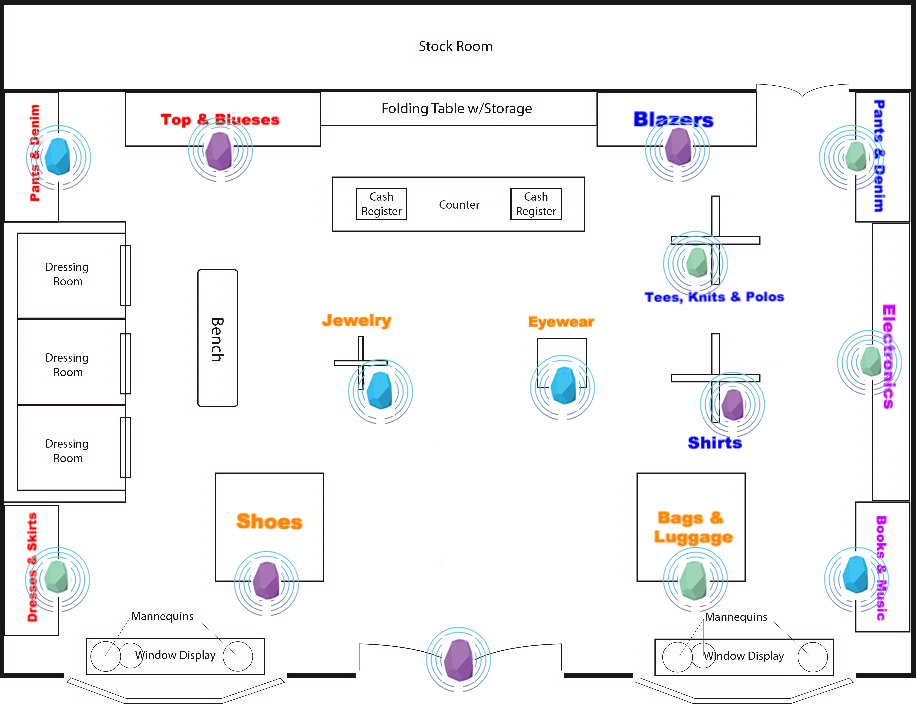
\includegraphics[width=16cm]{images/madison/retail-map-beacon.jpg}
  \caption{Madison Island retail store with Estimote beacons allocation}
  \label{fig:beacons-map}
\end{figure}
\vspace{0.5cm}

Depending on the business use case, the mobile app can wether send an event to the listening server whenever the user enters within each region boundary or submit a single event with a full list of regions detected during the staying along with their minimum proximities. 

Due to the behavioral profiling nature of this activity, we assume the app behaves like the latter and detects all the events entering or leaving each virtual fence activating a \textit{ranging} procedure aimed to detect proximity information based on the strenght of the Bluetooth signal. \cite{region-monitoring-apple}.

Once the shoppers leaves the retail store the app performs a single data push to a REST API endpoint with all the tracked data.

From a technical perspective, all these operations are accomplished leveraging the Estimote iOS-SDK \cite{estimote-ios-sdk} which allows the developer to define regions and ranges for each beacon quickly and facilitates the ranging process to track the actual proximity to them.

The JSON payload sent from the app to the REST endpoint for customer 3045678 (e.g. \textbf{POST /users/3045678/sessions}) for analysis would have this structure:


\vspace{0.5cm}
\begin{lstlisting}[language=json,firstnumber=1]
  {
    "data":{
       "customerId":3045678,
       "storeId":8784,
       "storeLabel" : "Madison1",
       "sessionId" : "89376f84-065b-11e8-ba89-0ed5f89f718b"
       "sessionDate": "2018-02-21",
       "sessionDuration" : 345,
       "sessionRegions":[
             {
                "regionId: : 156,
                "regionLabel":"store-entrance",
                "detectionCount":2,
                "maxSecondsInRegion": 5,
                "maxProximity":"unknown",
                "firstDetectionTimestamp":"2018-02-21T18:09:07Z",
                "lastDetectionTimestamp":"2018-02-21T18:16:02Z",
                "beaconData" : {
                  "uuid":"0686a88e-fed6-11e7-8be5-0ed5f89f718b",
                  "majorId":2553,
                  "minorId":79
                }
             },
             {
                "regionId: : 645,
                "regionLabel":"shoes",
                "detectionCount":1,
                "maxSecondsInRegion": 24,
                "maxProximity":"near",
                "firstDetectionTimestamp":"2018-02-21T18:09:20Z",
                "lastDetectionTimestamp":"2018-02-21T18:09:20Z",
                "beaconData" : {
                  "uuid":"0686a88e-fed6-11e7-8be5-0ed5f89f718b",
                  "majorId":19029,
                  "minorId":49
                }
             },
             {
                "regionId" : 6875,
                "regionLabel":"jewelry",
                "detectionCount":1,
                "maxSecondsInRegion": 15,
                "maxProximity":"far",
                "firstDetectionTimestamp":"2018-02-21T18:10:15Z",
                "lastDetectionTimestamp":"2018-02-21T18:10:15Z",
                "beaconData" : {
                  "uuid":"0686a88e-fed6-11e7-8be5-0ed5f89f718b",
                  "majorId":38415,
                  "minorId":59
                }
             },
             {
                "regionId" : 6875,
                "regionLabel":"blazers",
                "detectionCount":1,
                "maxSecondsInRegion": 195,
                "maxProximity":"immediate",
                "firstDetectionTimestamp":"2018-02-21T18:11:01Z",
                "lastDetectionTimestamp":"2018-02-21T18:11:01Z",
                "beaconData" : {
                  "uuid":"0686a88e-fed6-11e7-8be5-0ed5f89f718b",
                  "majorId":25911,
                  "minorId":27
                }
             },
             {
                "regionId" : 456,
                "regionLabel":"tees-knits-polos",
                "detectionCount":1,
                "maxSecondsInRegion": 10,
                "maxProximity":"far",
                "firstDetectionTimestamp":"2018-02-21T18:14:56Z",
                "lastDetectionTimestamp":"2018-02-21T18:14:56Z",
                "beaconData" : {
                  "uuid":"0686a88e-fed6-11e7-8be5-0ed5f89f718b",
                  "majorId":42037,
                  "minorId":36
                }
             },
             {
                "regionId" : 998,
                "regionLabel":"bags-and-luggage",
                "detectionCount":1,
                "maxSecondsInRegion": 7,
                "maxProximity":"far",
                "firstDetectionTimestamp":"2018-02-21T18:15:12Z",
                "lastDetectionTimestamp":"2018-02-21T18:15:12Z",
                "beaconData" : {
                  "uuid":"0686a88e-fed6-11e7-8be5-0ed5f89f718b",
                  "majorId":37931,
                  "minorId": 85
                }
             }
          ]
    }
 }
  \end{lstlisting}
\vspace{0.5cm}


The above example session shows an evident preference in "Blazer" items by the customer and a slight interest in the "Shoes" items. More precisely, the "Blazer" region registered a session lasted more than 3 minutes and the highest proximity to a beacon.  

\subsection{Customer Rewards}

Besides Proximity based marketing, Beacon technology can also be used to reward customers for particular actions based on geolocalization data improving the overall quality of the brand loyalty program which is key to cultivating lasting customer relationships. 

Achieving such result is possible by expanding the set of actions that enable customers to earn bonuses and discounts on the website (newsletter subscriptions, minimum order amount, etc..) to additional activities performed in the real world, including the simple act of visiting and walking around the store.

For example, the brand can rank customers by the amount of time spent at each Madison Retail shop and reward them with tailored offers every month depening on their purchases, or it can focus on offering special offers on the website to those customers that visited a retail store in a specific time span such as Christmas Time.

For our Madison Island example, we are considering a use case scenario where customers get rewarded if they manage to scan three products QR codes from the store to earn a fixed amount of reward points on their online account. Specifically, when the beacon detects their entrance into the store, the mobile app pushes a notification to the lock screen presenting a CheckPoints message to the customer inviting him to scan codes of actual items available in the shop. After each valid scan, the mobile app pushes the information about the scanned product to the same REST API used in the previous chapter which is responsible for storing the data.

\vspace{0.5cm}
\begin{figure}[H]
  \centering
    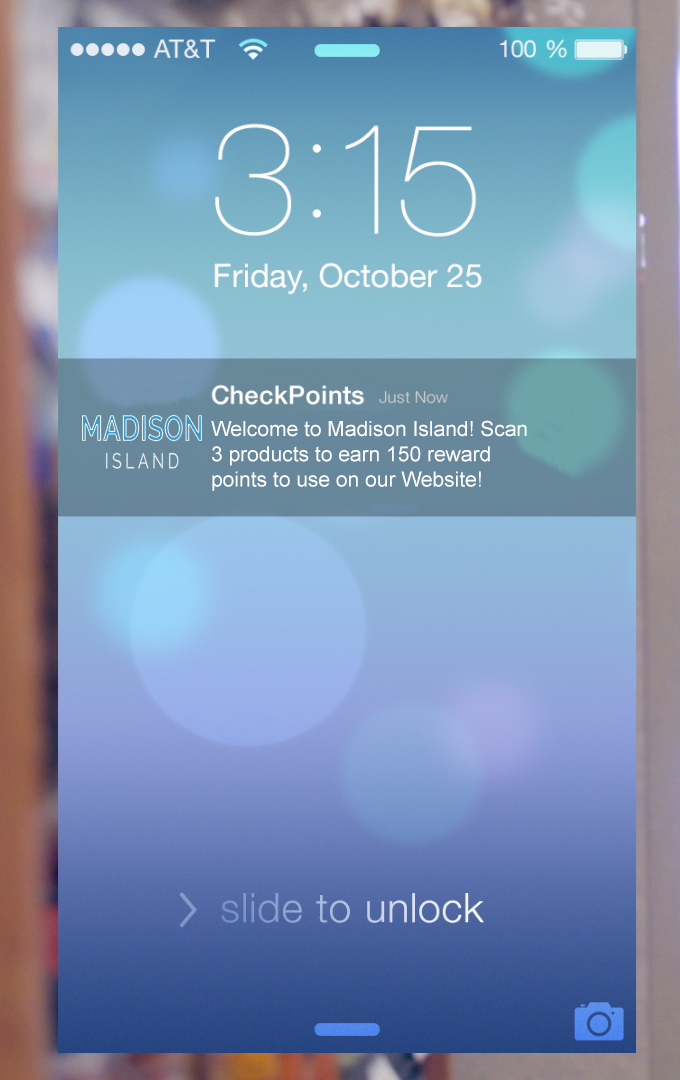
\includegraphics[width=8cm]{images/madison-push-reward-points.jpg}
  \caption{Madison Island mobile app push notification example}
  \label{fig:retail-map}
\end{figure}
\vspace{0.5cm}


The JSON payload sent to the server (e.g. \textbf{POST /users/3045678/scans}) after each succesful scan would then have a structure similar to this :

\vspace{0.5cm}
\begin{lstlisting}[language=json,firstnumber=1]
  {
    "data":{
       "customerId":3045678,
       "storeId":8784,
       "storeLabel" : "Madison1",
       "sessionId" : "89376f84-065b-11e8-ba89-0ed5f89f718b"
       "eventTime": "2018-02-21T18:11:02Z",
       "sessionActions": [{
          "userAgent" : "Iphone 6s",
          "scannedItems":
            {
              "barcode":"042100005264",
              "name" : "ELIZABETH KNIT TOP"
              "sku": "wbk012c"    
          }
      }]
    }
 }
  \end{lstlisting}
\vspace{0.5cm}

Similarly to the process outlined in \ref{ssection:proximity-marketing} the data collected by the server about each one of the single product scans performed by the customers during their sessions in the retail store will eventually convert in reward points attributions to use on the website for the customers. 

\vspace{0.5cm}
\begin{figure}[H]
  \centering
    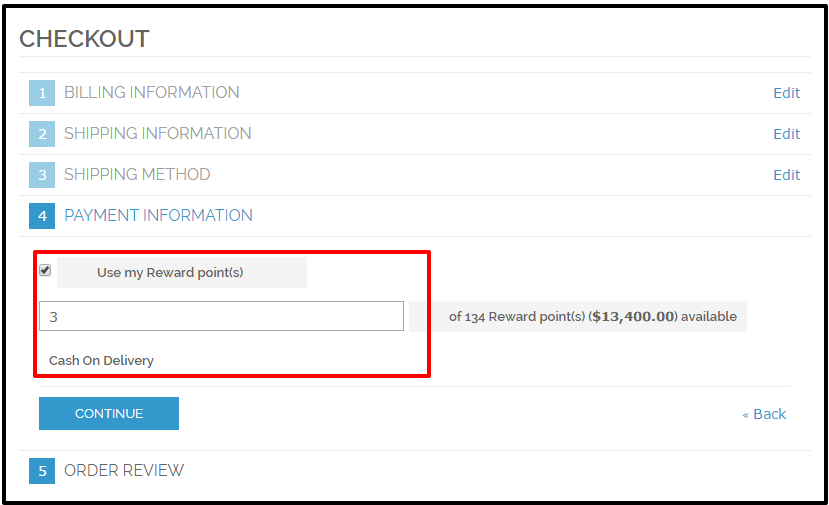
\includegraphics[width=12cm]{images/loyalty-reward-points.png}
  \caption{Madison Island loyalty program usage during checkout}
  \label{fig:loyalty-points}
\end{figure}
\vspace{0.5cm}





